\opengraphsfile{ApplicationsofExponentialandLogarithmicFunctions}

\setcounter{footnote}{0}

\label{ExpLogApplications}

As we mentioned in Sections \ref{ExponentialFunctions} and \ref{LogarithmicFunctions}, exponential and logarithmic functions are used to model a wide variety of behaviors in the real world.  In the examples that follow, note that while the applications are drawn from many different disciplines, the mathematics remains essentially the same.  Due to the applied nature of the problems we will examine in this section, we will often express our final answers as decimal approximations (after finding exact answers first, of course!)

\subsection{Applications of Exponential Functions}
\label{expapp}

Perhaps the most well-known application of exponential functions comes from the financial world.  Suppose you have $ \$ 100$ to invest at your local bank and they are offering a whopping $5 \, \%$ annual percentage interest rate.  This means that after one year, the bank will pay \textit{you} $5 \%$ of that $\$100$, or $ \$ 100(0.05) =\$ 5$ in interest, so you now have $\$105$. This is in accordance with the formula for  \textit{simple interest} which you have undoubtedly run across at some point before.

\smallskip

\colorbox{ResultColor}{\bbm

\begin{eqn} \index{interest ! simple} \index{simple interest} \label{simpleinterest} \textbf{Simple Interest:} 

The amount of interest $I$ accrued at an annual rate $r$ on an investment\footnote{Called the \index{principal} \textbf{principal}} $P$ after $t$ years is  \[I = Prt\]  The amount  in the account after $t$ years, $A(t)$ is given by \[A(t) = P + I = P + Prt = P(1+rt)\]

\end{eqn}

\ebm}
\smallskip

Suppose, however, that six months into the year, you hear of a better deal at a rival bank.\footnote{Some restrictions may apply.} Naturally, you withdraw your money and try to invest it at the higher rate there.  Since six months is one half of a year, that initial $\$100$ yields $\$100(0.05)\left(\frac{1}{2}\right) = \$ 2.50$ in interest.  

\smallskip

You take your $\$102.50$ off to the competitor and find out that those restrictions which \textit{may} apply actually \underline{do} apply, so you return to your bank and re-deposit the $\$102.50$ for the remaining six months of the year. 

\smallskip 

To your surprise and delight, at the end of the year your statement reads $\$105.06$, not $\$105$ as you had expected.\footnote{Actually, the final balance should be $\$105.0625$.}  Where did those extra six cents come from?  

\smallskip

For the first six months of the year, interest was earned on the original principal of $\$100$, but for the second six months, interest was earned on $\$102.50$, that is, you earned interest on your interest.  This is the basic concept behind \textbf{compound interest}. 

\smallskip

In the previous discussion, we would say that the interest was compounded twice per year, or semiannually.\footnote{Using this convention, simple interest after one year is the same as compounding the interest only once.}  If more money can be earned by earning interest on interest already earned, one wonders what happens if the interest is compounded more often, say every three months -  $4$ times a year, or `quarterly.' 

\smallskip

In this case, the money is in the account for three months, or $\frac{1}{4}$ of a year, at a time.  After the first quarter, we have $A = P(1+rt) =  \$100 \left(1 + 0.05 \cdot \frac{1}{4} \right) = \$101.25$.  We now invest the $\$101.25$ for the next three months and find that at the end of the second quarter, we have $A =  \$101.25 \left(1 + 0.05 \cdot \frac{1}{4} \right)\approx \$102.51$.  Continuing in this manner, the balance at the end of the third quarter is $\$103.79$, and, at last, we obtain $\$105.08$.  The extra two cents hardly seems worth it, but we see that we do in fact get more money the more often we compound. 

\smallskip

In order to develop a formula for this phenomenon, we need to do some abstract calculations.  Suppose we wish to invest our principal $P$ at an annual rate $r$ and compound the interest $n$ times per year.  This means the money sits in the account $\frac{1}{n}^{\mbox{\tiny th}}$ of a year between compoundings.  Let $A_{k}$ denote the amount in the account after the $k^{\mbox{\tiny th}}$ compounding. 

\smallskip

Then $A_{\mbox{\tiny$1$}} = P\left(1 + r\left(\frac{1}{n}\right)\right)$ which simplifies to $A_{\mbox{\tiny$1$}} = P \left(1 + \frac{r}{n}\right)$.  After the second compounding, we use $A_{\mbox{\tiny$1$}}$ as our new principal and get $A_{\mbox{\tiny$2$}} = A_{\mbox{\tiny$1$}} \left(1 + \frac{r}{n}\right) = \left[P \left(1 + \frac{r}{n}\right)\right]\left(1 + \frac{r}{n}\right) = P \left(1 + \frac{r}{n}\right)^2$.  Continuing in this fashion, we get $A_{\mbox{\tiny$3$}} =P \left(1 + \frac{r}{n}\right)^3$, $A_{\mbox{\tiny$4$}} =P \left(1 + \frac{r}{n}\right)^4$, and so on, so that $A_{k} = P \left(1 + \frac{r}{n}\right)^k$.  

\smallskip

Since we compound the interest $n$ times per year, after $t$ years, we have $nt$ compoundings. We have just derived the general formula for compound interest below.

\smallskip

\colorbox{ResultColor}{\bbm

\begin{eqn} \index{interest ! compound} \index{compound interest} \label{compoundinterest} \textbf{Compounded Interest:}  

If an initial principal $P$ is invested at an annual rate $r$ and the interest is compounded $n$ times per year, the amount in the account after $t$ years, $A(t)$  is given by \[A(t) = P \left(1 + \frac{r}{n}\right)^{nt}\]

\end{eqn}

\ebm}

\smallskip

If we take $P = 100$, $r = 0.05$, and $n = 4$, Equation \ref{compoundinterest} becomes $A(t) = 100\left(1+ \frac{0.05}{4}\right)^{4t}$ which reduces to $A(t) = 100(1.0125)^{4t}$.  To check this new formula against our previous calculations, we find $A\left(\frac{1}{4}\right) = 100(1.0125)^{4 \left(\frac{1}{4}\right)} = 101.25$, $A\left(\frac{1}{2}\right) \approx \$102.51$, $A\left(\frac{3}{4}\right) \approx \$103.79$, and $A(1) \approx \$105.08$.

\begin{ex}  \label{compoundinterestex} Suppose $\$2000$ is invested in an account which offers $7.125 \%$ compounded monthly.

\begin{enumerate}

\item Express the amount $A(t)$ in the account as a function of the term of the investment $t$ in years.

\item  How much is in the account after $5$ years? 

\item  How long will it take for the initial investment to double?

\item  Find and interpret the average rate of change\footnote{See Definition \ref{arc} in Section \ref{ConstantandLinearFunctions}.} of the amount in the account:

\begin{itemize}

\item  from the end of the fourth year to the end of the fifth year

\item from the end of the thirty-fourth year to the end of the thirty-fifth year.

\end{itemize}

\pagebreak

\item  Find and interpret the relative rate of change\footnote{See Definition \ref{rrc} in Section \ref{ExponentialFunctions}.} of the amount in the account: 

\begin{itemize}

\item  from the end of the fourth year to the end of the fifth year

\item from the end of the thirty-fourth year to the end of the thirty-fifth year.

\end{itemize}

\end{enumerate}

{\bf Solution.}  

\begin{enumerate}

\item  Substituting $P = 2000$, $r = 0.07125$, and $n = 12$ (since interest is compounded \textit{monthly}) into Equation \ref{compoundinterest} yields $A(t) = 2000\left(1 + \frac{0.07125}{12}\right)^{12t}=2000 (1.0059375)^{12t}$.

\item  To find the amount in the account after $5$ years, we compute $A(5) = 2000 (1.0059375)^{12(5)} \approx 2852.92$.  After $5$ years, we have approximately $\$2852.92$.

\item  Our initial investment is $\$2000$, so to find the time it takes this to double, we need to find $t$ when $A(t) = 4000$.  That is, we need to solve $2000 (1.0059375)^{12t}=4000$, or $(1.0059375)^{12t}=2$.  

\smallskip

Taking natural logs as in Section \ref{ExponentialEquationsandInequalities}, we get $t = \frac{\ln(2)}{12 \ln(1.0059375)} \approx 9.75$.  Hence, it takes approximately $9$ years $9$ months for the investment to double.

\item  Recall to find the average rate of change of $A$ over an interval $[a,b]$, we compute $\frac{A(b)-A(a)}{b-a}$.

\begin{itemize}

\item  The average rate of change of $A$  from the end of the fourth year to the end of the fifth year is $\frac{A(5)-A(4)}{5-4} \approx 195.63$.  

\smallskip

This means that the value of the investment is increasing at a rate of approximately $\$195.63$ per year between the end of the fourth and fifth years.

\item  Likewise, the average rate of change of $A$  from the end of the thirty-fourth year to the end of the thirty-fifth year is $\frac{A(35)-A(34)}{35-34} \approx 1648.21$, so the value of the investment is increasing at a rate of approximately $\$1648.21$ per year during this time.

\end{itemize}

So, not only is it true that the longer you wait, the more money you have, but also the longer you wait, the faster the money increases.\footnote{In fact, the rate of increase of the amount in the account is exponential as well.  This is the quality that really defines exponential functions and we refer the reader to a course in Calculus.} 

\item    Recall to find the relative rate of change of $A$ over an interval $[a,b]$, we compute $\frac{A(b)-A(a)}{A(a)}$.

\begin{itemize}

\item  The relative rate of change of $A$ from the end of the fourth year to the end of the fifth year is $\frac{A(5)-A(4)}{A(4)} \approx 0.07362$. 

\smallskip

This means that the amount in the account is increasing at a rate of approximately $7.362 \%$ per year between the end of the fourth and fifth years.

\item Similarly, we find the relative rate of change of $A$ from the end  of the thirty-fourth year to the end of the thirty-fifth year to be $\frac{A(35)-A(34)}{A(34)} \approx  0.07362$ as well.  

This means that the percentage growth from the thirty-fourth to thirty-fifth year is $7.362 \%$, the same as the percentage growth from the fourth to the fifth year.

\end{itemize}

We know from the remarks following Definition \ref{rrc} that for exponential functions, the relative rate of change over an interval of length $1$ is constant and, moreover, is equal to $b-1$ where $b$ is the base of the exponential function, $f(x) = a \cdot b^{x}$.  

\smallskip

In our scenario,  $A(t) = 2000 (1.0059375)^{12t} = 2000  \left[(1.0059375)^{12}\right]^{t} = 2000 \cdot (1.07362 \ldots)^t$.  Hence, the base is $b = 1.07362 \ldots$ and the relative rate of change is $b-1 = 0.07362 \ldots$.    

\smallskip

Note that the interest rate quoted to us at the beginning of this problem is $7.125 \%$ per year.  The rate $7.362 \%$ is called the `\textit{effective}' interest rate which factors in the effect of the compounding on the growth of the investment. \qed

\end{enumerate}

\end{ex}

We have observed that the more times you compound the interest per year, the more money you will earn in a year.  Let's push this notion to the limit.\footnote{Once you've had a semester of Calculus, you'll be able to fully appreciate this very lame pun.}  

\smallskip

Consider an investment of $\$ 1$ invested at $100 \%$ interest for $1$ year compounded $n$ times a year.  Equation \ref{compoundinterest} tells us that the amount of money in the account after $1$ year is $A = \left(1+\frac{1}{n}\right)^{n}$.  Below is a table of values relating $n$ and $A$.

\[ \begin{array}{|r||r|}  

\hline

 n & A   \\ \hline
1  & 2  \\  \hline
2  & 2.25  \\  \hline
4 & \approx 2.4414  \\  \hline
12 & \approx 2.6130  \\  \hline
360  & \approx  2.7145 \\  \hline
1000  & \approx 2.7169 \\  \hline
10000  & \approx 2.7181  \\  \hline
100000 & \approx 2.7182  \\  \hline
\end{array} \]

As promised, the more compoundings per year, the more money there is in the account, but we also observe that the increase in money is greatly diminishing.  

\smallskip

We are witnessing a mathematical `tug of war'.  While we are compounding more times per year, and hence getting interest on our interest more often, the amount of time between compoundings is getting smaller and smaller, so there is less time to build up additional interest. 

\smallskip

With Calculus, we can show\footnote{Or define, depending on your point of view.} that as $n \rightarrow \infty$, $A = \left(1+\frac{1}{n}\right)^{n} \rightarrow e$, where $e$ is the natural base first presented in Section \ref{ExponentialFunctions}.  Taking the number of compoundings per year to infinity results in what is called  \textbf{continuously} compounded interest.  

\smallskip

\colorbox{ResultColor}{\bbm

\begin{thm} \label{whatise} Investing $\$1$ at $100 \%$ interest compounded continuously for one year returns $\$ e$. 

\end{thm}

\ebm}

\smallskip

Using this definition of $e$ and a little Calculus, we can take Equation \ref{compoundinterest} and produce a formula for continuously compounded interest.

\smallskip

\colorbox{ResultColor}{\bbm

\begin{eqn} \index{interest ! compounded continuously} \index{continuously compounded interest} \label{continuouscompoundinterest} \textbf{Continuously Compounded Interest:} 

If an initial principal $P$ is invested at an annual rate $r$ and the interest is compounded continuously, the amount  in the account after $t$ years, $A(t)$ is given by  \[A(t) = P e^{rt} \]

\end{eqn}

\ebm}

\smallskip

If we take the scenario of Example \ref{compoundinterestex} and compare monthly compounding to continuous compounding over $35$ years, we find that monthly compounding yields $A(35) = 2000 (1.0059375)^{12(35)}$ which is about  $\$ 24,\!035.28$, whereas continuously compounding gives $A(35) = 2000e^{0.07125 (35)}$ which is about  $\$ 24,\!213.18$ - a difference of less than $1 \%$.

\smallskip

Equations \ref{compoundinterest} and \ref{continuouscompoundinterest} both use exponential functions to describe the growth of an investment.  It turns out, the same principles which govern compound interest are also used to model short term growth of populations.  As with many concepts in this text, these notions are best formalized using the language of Calculus.  Nevertheless, we do our best here.  

\smallskip

In Biology, \textbf{The Law of Uninhibited Growth} states as its premise that the \textit{instantaneous} \index{instantaneous rate of change} \index{rate of change ! instantaneous} rate at which a population increases at any time is directly proportional to the population at that time.\footnote{The average rate of change of a function over an interval was first introduced in Section \ref{ConstantandLinearFunctions}.  The notion of \textit{instantaneous} rate of change was introduced in the remarks following Example \ref{ARCRocketExample} and revisited in Example \ref{averagevelocityrocketex}.}  In other words, the more organisms there are at a given moment, the faster they reproduce.  Formulating the law as stated results in a differential equation, which requires Calculus to solve.  Solving said differential equation gives us the formula below.

\smallskip

\colorbox{ResultColor}{\bbm

\begin{eqn} \index{growth model ! uninhibited} \index{uninhibited growth} \label{lawofuninhibitedgrowth} \textbf{Uninhibited Growth:} 

If a population increases according to The Law of Uninhibited Growth, the number of organisms at time $t$, $N(t)$  is given by the formula  \[N(t) = N_{\mbox{\tiny$0$}}e^{kt},\] where $N(0) = N_{\mbox{\tiny$0$}}$ (read `$N$ nought') is the initial number of organisms and $k>0$ is the constant of proportionality which satisfies the equation:

\[ \left(\mbox{instantaneous rate of change of $N(t)$ at time $t$}\right) = k \, N(t)\]

\smallskip

\end{eqn}

\ebm}

\smallskip 

 It is worth taking some time to compare Equations \ref{continuouscompoundinterest} and \ref{lawofuninhibitedgrowth}.  In  Equation \ref{continuouscompoundinterest}, we use $P$ to denote the initial investment;  in Equation \ref{lawofuninhibitedgrowth}, we use $N_{\mbox{\tiny$0$}}$ to denote the initial population.  In  Equation \ref{continuouscompoundinterest}, $r$ denotes the annual interest rate,  and so it shouldn't be too surprising that the $k$ in Equation \ref{lawofuninhibitedgrowth} corresponds to a growth rate as well.   While Equations \ref{continuouscompoundinterest} and \ref{lawofuninhibitedgrowth} look entirely different, they both represent the same mathematical concept.

\smallskip

\begin{ex}  In order to perform arthrosclerosis research, epithelial cells are harvested from discarded umbilical tissue and grown in the laboratory.  A technician observes that a culture of twelve thousand cells grows to five million cells in one week.  Assuming that the cells follow The Law of Uninhibited Growth, find a formula for the number of cells, in thousands, after $t$ days, $N(t)$.

\smallskip

{\bf Solution.}  We begin with $N(t) = N_{\mbox{\tiny$0$}}e^{kt}$.  Since $N(t)$ is to give the number of cells \textit{in thousands}, we have $N_{\mbox{\tiny$0$}} = 12$, so $N(t) = 12e^{kt}$. 

Next, we need to determine the growth rate $k$.  We know that after one week, the number of cells has grown to five million.  Since $t$ measures days and the units of $N(t)$ are in thousands, this translates mathematically to $N(7) = 5000$ or  $12e^{7k} = 5000$.   Solving, we get $k = \frac{1}{7} \ln\left(\frac{1250}{3}\right)$, so  $N(t) = 12e^{ \frac{t}{7} \ln\left(\frac{1250}{3}\right)}$.  

\smallskip

Of course, in practice, we would approximate $k$ to some desired accuracy, say $k \approx 0.8618$, which we can interpret as an $86.18 \%$ daily growth rate for the cells. \qed

\end{ex}

Whereas Equations \ref{continuouscompoundinterest} and \ref{lawofuninhibitedgrowth} model the growth of quantities, we can use equations like them to describe the decline of quantities.  

\smallskip

One example we've seen already is Example \ref{cardepreciationex} in Section \ref{ExponentialFunctions}.  There, the value of a car decreased from its purchase price of $\$25,\!000$ to nothing at all.  

\smallskip

Another real world phenomenon which follows suit is radioactive decay.  There are elements which are unstable and emit energy spontaneously.  In doing so, the amount of the element itself diminishes.  

\smallskip

The assumption behind this model is that the rate of decay of an element at a particular time is directly proportional to the amount of the element present at that time.  In other words, the more of the element there is, the faster the element decays.  

\smallskip

This is precisely the same kind of hypothesis which drives The Law of Uninhibited Growth, and as such, the equation governing radioactive decay is hauntingly similar to Equation \ref{lawofuninhibitedgrowth} with the exception that the rate constant $k$ is negative.

\smallskip

\colorbox{ResultColor}{\bbm

\begin{eqn} \index{radioactive decay} \label{radioactivedecay} \textbf{Radioactive Decay:}

 The amount of a radioactive element  at time $t$, $A(t)$ is given by the formula  \[A(t) = A_{\mbox{\tiny$0$}}e^{kt},\] where $A(0) = A_{\mbox{\tiny$0$}}$ is the initial amount of the element and  $k<0$ is the constant of proportionality which satisfies the equation

\[ \left(\mbox{instantaneous rate of change of $A(t)$ at time $t$}\right) = k \, A(t)\]


\end{eqn}

\ebm}

\smallskip 

\begin{ex}  Iodine-131 is a commonly used radioactive isotope used to help detect how well the thyroid is functioning.  Suppose the decay of Iodine-131 follows the model given in Equation \ref{radioactivedecay}, and that the  half-life\footnote{The time it takes for half of the substance to decay.} of Iodine-131 is approximately $8$ days.  If $5$ grams of Iodine-131 is present initially, find a function which gives the amount of Iodine-131, $A$, in grams, $t$ days later.

\smallskip

{\bf Solution.} Since we start with $5$ grams initially, Equation \ref{radioactivedecay} gives $A(t) = 5e^{kt}$.  

\smallskip

Since the half-life is $8$ days, it takes $8$ days for half of the Iodine-131 to decay, leaving half of it behind.  Mathematically, this translates to  $A(8) = 2.5$, or $5e^{8k} = 2.5$.  We get $k = \frac{1}{8} \ln\left(\frac{1}{2}\right) = -\frac{\ln(2)}{8} \approx -0.08664$, which we can interpret as a loss of material at a rate of $8.664 \%$ daily.  

\smallskip

Hence, our final answer is $A(t) = 5 e^{-\frac{t\ln(2)}{8}} \approx 5 e^{-0.08664t}$. \qed

\end{ex}


We now turn our attention to some more mathematically sophisticated models.  One such model is Newton's Law of Cooling, which we first encountered in Example \ref{exptempex} of Section \ref{ExponentialFunctions}.   

\smallskip

In that example we had a cup of coffee cooling from $160^{\circ}\mbox{F}$ to room temperature $70^{\circ}\mbox{F}$ according to the formula $T(t) = 70 + 90 e^{-0.1 t}$, where $t$ was measured in minutes.  In that situation, we knew the physical limit of the temperature of the coffee was room temperature,\footnote{The Second Law of Thermodynamics states that heat can spontaneously flow from a hotter object to a colder one, but not the other way around.  Thus, the coffee could not continue to release heat into the air so as to cool below room temperature.} and the differential equation which gives rise to our formula for $T(t)$ takes this into account.  

\smallskip

Whereas the radioactive decay model had a rate of decay at time $t$ directly proportional to the amount of the element which remained at time $t$, Newton's Law of Cooling states that the rate of cooling of the coffee at a given time $t$ is directly proportional to how much of a temperature \textit{gap} exists between the coffee at time $t$ and room temperature, not the temperature of the coffee itself.  In other words, the coffee cools faster when it is first served, and as its temperature nears room temperature, the coffee cools ever more slowly.

\smallskip

 Of course, if we take an item from the refrigerator and let it sit out in the kitchen, the object's temperature will rise to room temperature, and since the physics behind warming and cooling is the same, we combine both cases in the equation below.

\smallskip

\colorbox{ResultColor}{\bbm

\begin{eqn} \index{Newton's Law of Cooling} \label{newtonslawofcooling} \textbf{Newton's Law of Cooling (Warming):}  

The temperature of an object  at time $t$, $T(t)$ is given by the formula \[T(t) = T_{a} + \left(T_{\mbox{\tiny$0$}} - T_{a}\right) e^{-kt},\] where $T(0) = T_{\mbox{\tiny$0$}}$ is the initial temperature of the object, $T_{a}$ is the ambient temperature\footnote{That is, the temperature of the surroundings.} and $k>0$ is the constant of proportionality which satisfies the equation

\[ \left(\mbox{instantaneous rate of change of $T(t)$ at time $t$}\right) = k \, \left(T(t) - T_{a}\right)\]



\end{eqn}

\ebm}

\smallskip 

If we re-examine the situation in Example \ref{exptempex} with $T_{\mbox{\tiny$0$}} = 160$, $T_{a} = 70$, and $k = 0.1$, we get, according to Equation \ref{newtonslawofcooling}, $T(t) = 70 + (160 - 70)e^{-0.1t}$ which reduces to the original formula given in that example.  The rate constant $k = 0.1$ in this case indicates the coffee is cooling at a rate equal to $10 \%$ of the difference between the temperature of the coffee and its surroundings.  

\smallskip

Note in Equation \ref{newtonslawofcooling} that the constant $k$ is positive for both the cooling and warming scenarios.  What determines if the function $T(t)$ is increasing or decreasing is if $T_{\mbox{\tiny$0$}}$ (the initial temperature of the object) is greater than $T_{a}$ (the ambient temperature) or vice-versa, as we see in our next example.

\smallskip

\begin{ex} \label{exptempex2} A roast initially at  $40^{\circ}\mbox{F}$ cooked in a $350^{\circ}\mbox{F}$ oven.  After $2$ hours, the temperature of the roast is $125^{\circ}\mbox{F}$.

\begin{enumerate}

\item  Assuming the temperature of the roast follows Newton's Law of Warming, find a formula for the temperature of the roast $T(t)$ as a function of its time in the oven, $t$, in hours.

\item  The roast is done when the internal temperature reaches $165^{\circ}\mbox{F}$.  When will the roast be done?

\end{enumerate}

\pagebreak

{\bf Solution.}

\begin{enumerate}

\item  The initial temperature of the roast is $40^{\circ}\mbox{F}$, so $T_{\mbox{\tiny$0$}} = 40$.  The environment in which we are placing the roast is the $350^{\circ}\mbox{F}$ oven, so $T_{a} = 350$. Newton's Law of Warming gives $T(t) = 350 + (40-350)e^{-kt}$, or after some simplification,  $T(t) = 350 - 310e^{-kt}$.  

\smallskip

To determine $k$, we use the fact that after $2$ hours, the roast is  $125^{\circ}\mbox{F}$, which means $T(2) = 125$.  This gives rise to the equation $350 - 310e^{-2k} = 125$ which yields $k = -\frac{1}{2} \ln \left( \frac{45}{62}  \right) \approx 0.1602$.  The temperature function is \[T(t) = 350 - 310 e^{\frac{t}{2} \ln \left( \frac{45}{62}  \right)} \approx 350- 310 e^{-0.1602 t}.\]


\item  To find when the roast is done, we set $T(t) = 165$.  This gives $350- 310 e^{-0.1602 t} = 165$ whose solution is $t = -\frac{1}{0.1602} \ln \left( \frac{37}{62}  \right) \approx 3.22$.  Hence, the roast is done after roughly $3$ hours and $15$ minutes. \qed

\end{enumerate}

\end{ex}

If we had taken the time to graph $y=T(t)$ in Example \ref{exptempex2}, we would have found the horizontal asymptote to be $y = 350$, which corresponds to the temperature of the oven. We can also arrive at this conclusion analytically by applying  `number sense'.  

\smallskip

As $t \rightarrow \infty$, $-0.1602 t \approx \mbox{very big $(-)$}$ so that $e^{-0.1602 t} \approx \mbox{very small $(+)$}$.  The larger the value of $t$, the smaller $e^{-0.1602 t}$ becomes so that $T(t) \approx 350 -\mbox{very small $(+)$}$, which indicates the graph of $y=T(t)$ is approaching its horizontal asymptote $y=350$ from below.   Physically, this means the roast will eventually warm up to $350^{\circ}\mbox{F}$.\footnote{at which point it would be more toast than roast.}  

\smallskip

The function $T$  in this situation is sometimes called a \index{growth model ! limited} \textbf{limited} growth model, since the function $T$ remains bounded as $t \rightarrow \infty$.  If we apply the principles behind Newton's Law of Cooling to a biological example, it says the growth rate of a population is directly proportional to how much room the population has to grow.  In other words, the more room for expansion, the faster the growth rate. 

\smallskip

Our final model, the \textbf{logistic} growth model combines The Law of Uninhibited Growth with limited growth and states that the rate of growth of a population varies jointly with the population itself as well as the room the population has to grow.   


\smallskip

\colorbox{ResultColor}{\bbm

\begin{eqn} \index{growth model ! logistic} \index{logistic growth} \label{logisticgrowth} \textbf{Logistic Growth:}  

If a population behaves according to the assumptions of logistic growth, the number of organisms at time $t$, $N(t)$  is given by  \[N(t) =\dfrac{L}{1 + Ce^{-kLt}},\] where $N(0) = N_{\mbox{\tiny$0$}}$ is the initial population,  $L$ is the limiting population,\footnote{That is, as $t \rightarrow \infty$, $N(t) \rightarrow L$} and $C$ is a measure of how much room there is to grow given by \[C = \dfrac{L}{N_{\mbox{\tiny$0$}}} - 1.\] and $k > 0$ is the constant of proportionality which satisfies the equation

\[ \left(\mbox{instantaneous rate of change of $N(t)$ at time $t$}\right) = k \, N(t) \left(L - N(t)\right)\]


\end{eqn}

\ebm}

\smallskip 

The logistic function is used not only to model the growth of organisms, but is also often used to model the spread of disease and rumors.\footnote{Which can be just as damaging as diseases.}

\smallskip

\begin{ex} \label{rumorex} The number of people $N(t)$, in hundreds, at a local community college who have heard the rumor `Carl's afraid of Sasquatch' can be modeled using the logistic equation

\[N(t) = \dfrac{84}{1+2799e^{-t}},\]

where $t\geq 0$ is the number of days after April 1, 2016.


\begin{enumerate}

\item  Find and interpret $N(0)$.

\item  \label{ebrumorex} Find and interpret the end behavior of $N(t)$. 

\item  \label{whenrumorex} How long until $4200$ people have heard the rumor?

\item  Check your answers to \ref{ebrumorex} and \ref{whenrumorex} using a graphing utility.

\end{enumerate}

{\bf Solution.}  

\begin{enumerate}

\item  We find $N(0) = \frac{84}{1+2799e^{0}} = \frac{84}{2800} = 0.03$.  Since $N(t)$ measures the number of people who have heard the rumor in hundreds, $N(0)$ corresponds to $3$ people.  Since $t=0$ corresponds to April 1, 2016, we may conclude that on that day, $3$ people have heard the rumor.\footnote{Or, more likely, three people started the rumor.  I'd wager Jeffey, Rosie, and JT started it.} 

\item  We could simply note that $N(t)$ is written in the form of Equation \ref{logisticgrowth}, and identify $L = 84$.  However, to see better \textit{why} the answer is $84$, we proceed analytically.  

Since the domain of $N$ is restricted to $t \geq 0$, the only end behavior of significance is $t \rightarrow \infty$. As we've seen before,\footnote{See, for example, Example \ref{exptempex}.} as $t \rightarrow \infty$, we have $1997 e^{-t} \rightarrow 0^{+}$ and so $N(t) \approx \frac{84}{1 + \text{\scriptsize very small $(+)$}} \approx 84$.  

Hence, as $t \rightarrow \infty$, $N(t) \rightarrow 84$.   This means that as time goes by, the number of people who will have heard the rumor approaches $8400$. 

\item  To find how long it takes until $4200$ people have heard the rumor, we set $N(t) = 42$.  Solving $\frac{84}{1+2799e^{-t}} = 42$ gives $t =  \ln(2799) \approx 7.937$, so   it takes around $8$ days until $4200$ people have heard the rumor.

\item  Graphing $y=N(t)$ below, we see $y=84$ is the horizontal asymptote of the graph, confirming our answer to number  \ref{ebrumorex}, and the graph intersects the line $y=42$ at $t \approx 7.937 \approx \ln(2799) $, which confirms our answer to number \ref{whenrumorex}.

\begin{center}

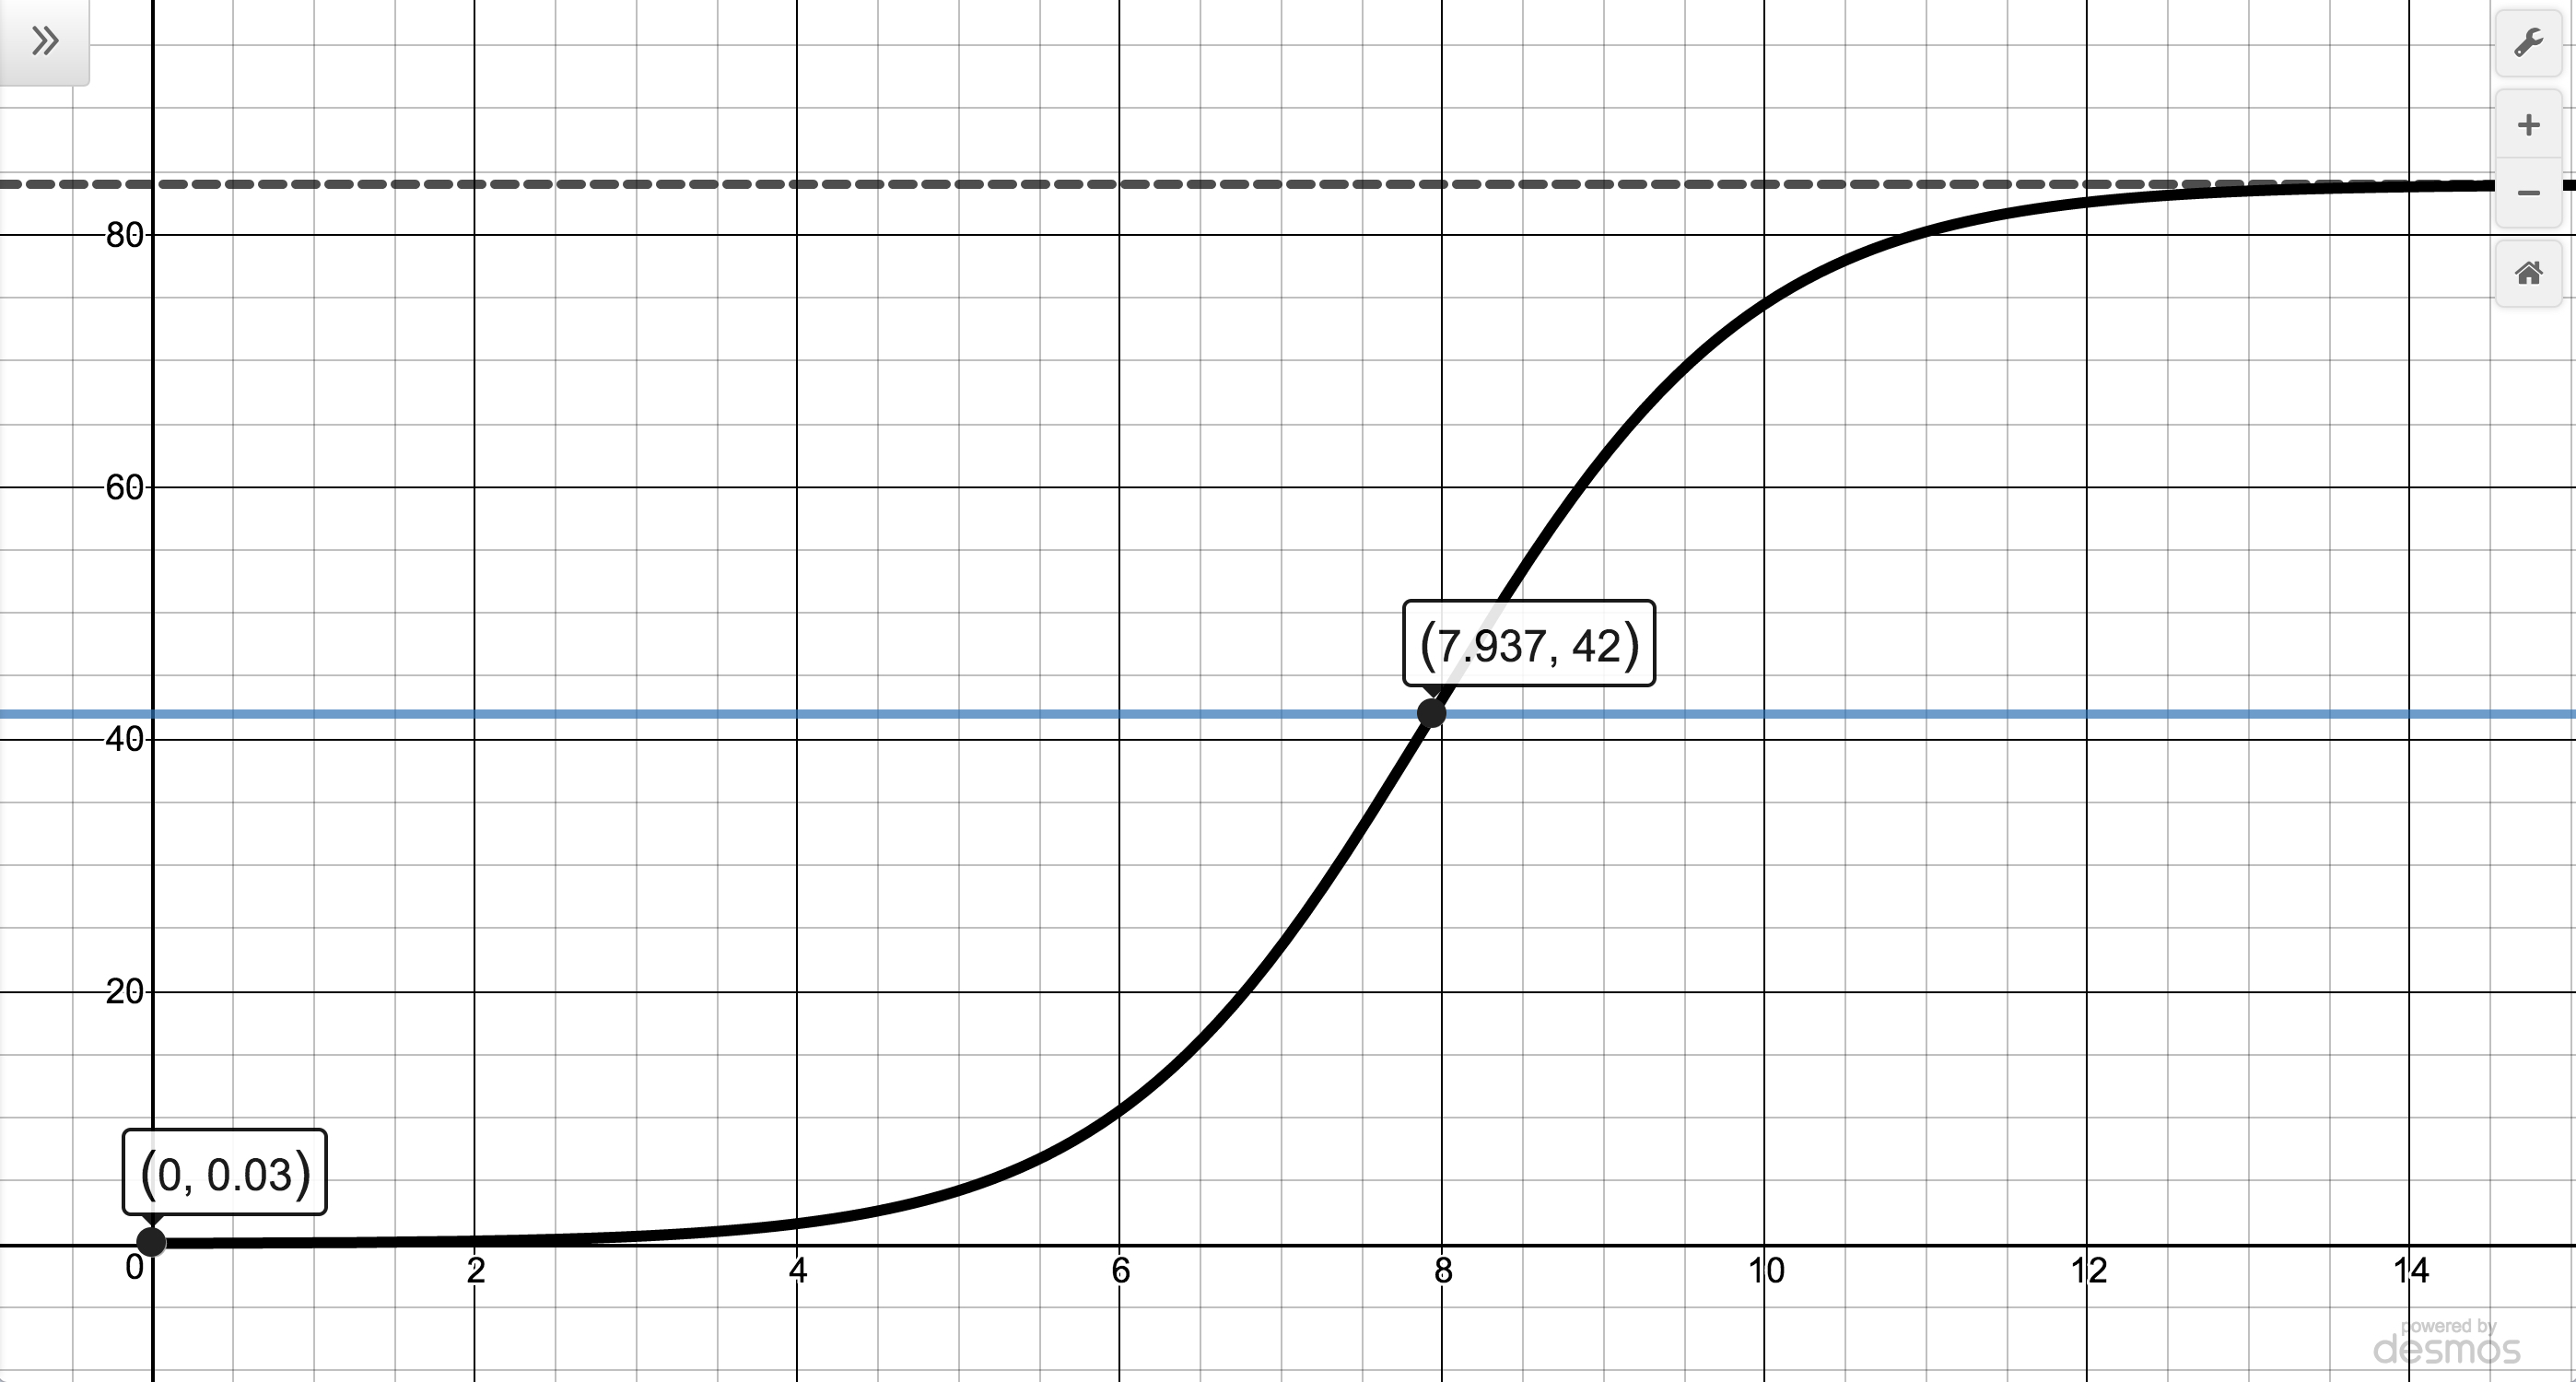
\includegraphics[width=4in]{./ApplicationsofExponentialandLogarithmicFunctionsGraphics/ExpLogAppEx01.jpg} 


\end{center}

\end{enumerate}

\qed

\end{ex}

If we take the time to analyze the graph of $y=N(t)$ in Example \ref{rumorex}, we can see \textit{graphically} how logistic growth combines  features of uninhibited and limited growth.  

\smallskip

The curve is concave up, rising steeply, then at some point, becomes concave down and begins to level off.\footnote{We introduced the notion of concavity in Section \ref{PowerFunctions}.}  The point at which this happens is called an \index{inflection point}\index{point of diminishing returns} \textbf{inflection point} or is sometimes called the `point of diminishing returns'.   Even though the function is still increasing through the inflection point, the \textit{rate} at which it does so begins to decrease. 

\smallskip

With Calculus, one can show the point of diminishing returns always occurs at half the limiting population.  (In our case, when $N(t)=42$.)  So with that in mind, we present two portions of the graph of $y=N(x)$, one on the interval $[0,8]$, the other on $[8,15]$. The former looks strikingly like uninhibited growth while the latter like limited growth.

\begin{center}

\begin{tabular}{cc}

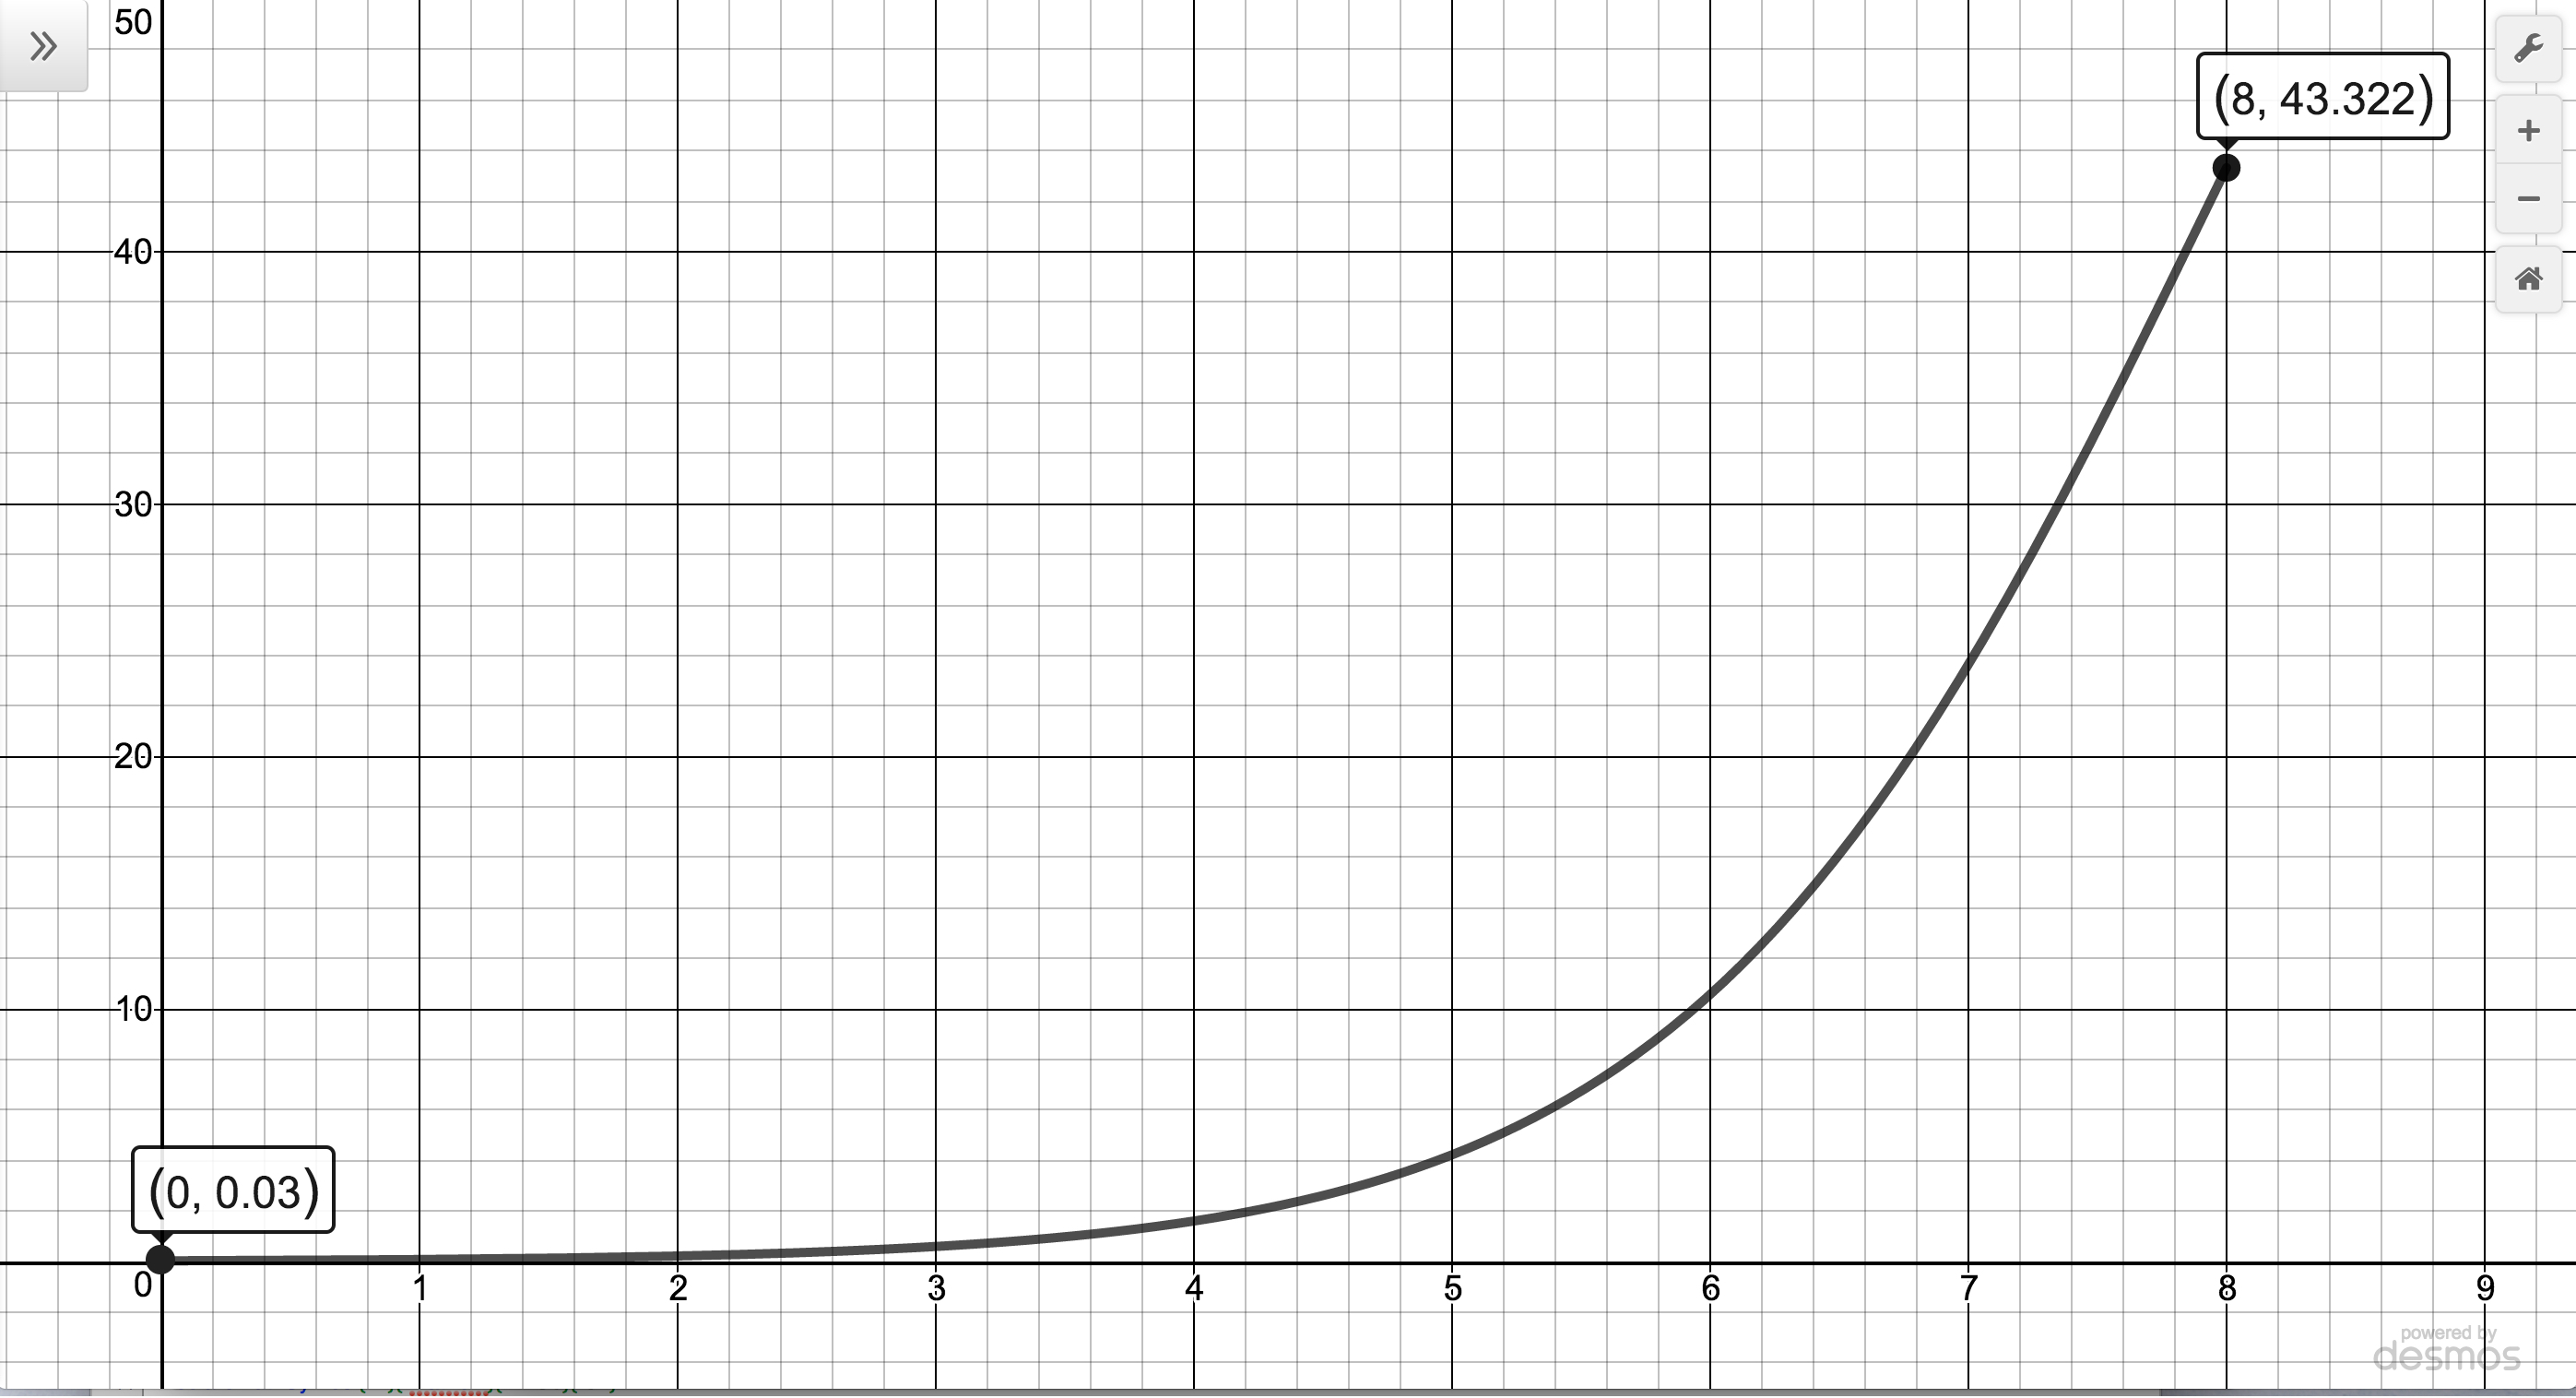
\includegraphics[width=3in]{./ApplicationsofExponentialandLogarithmicFunctionsGraphics/ExpLogAppEx02.jpg} &

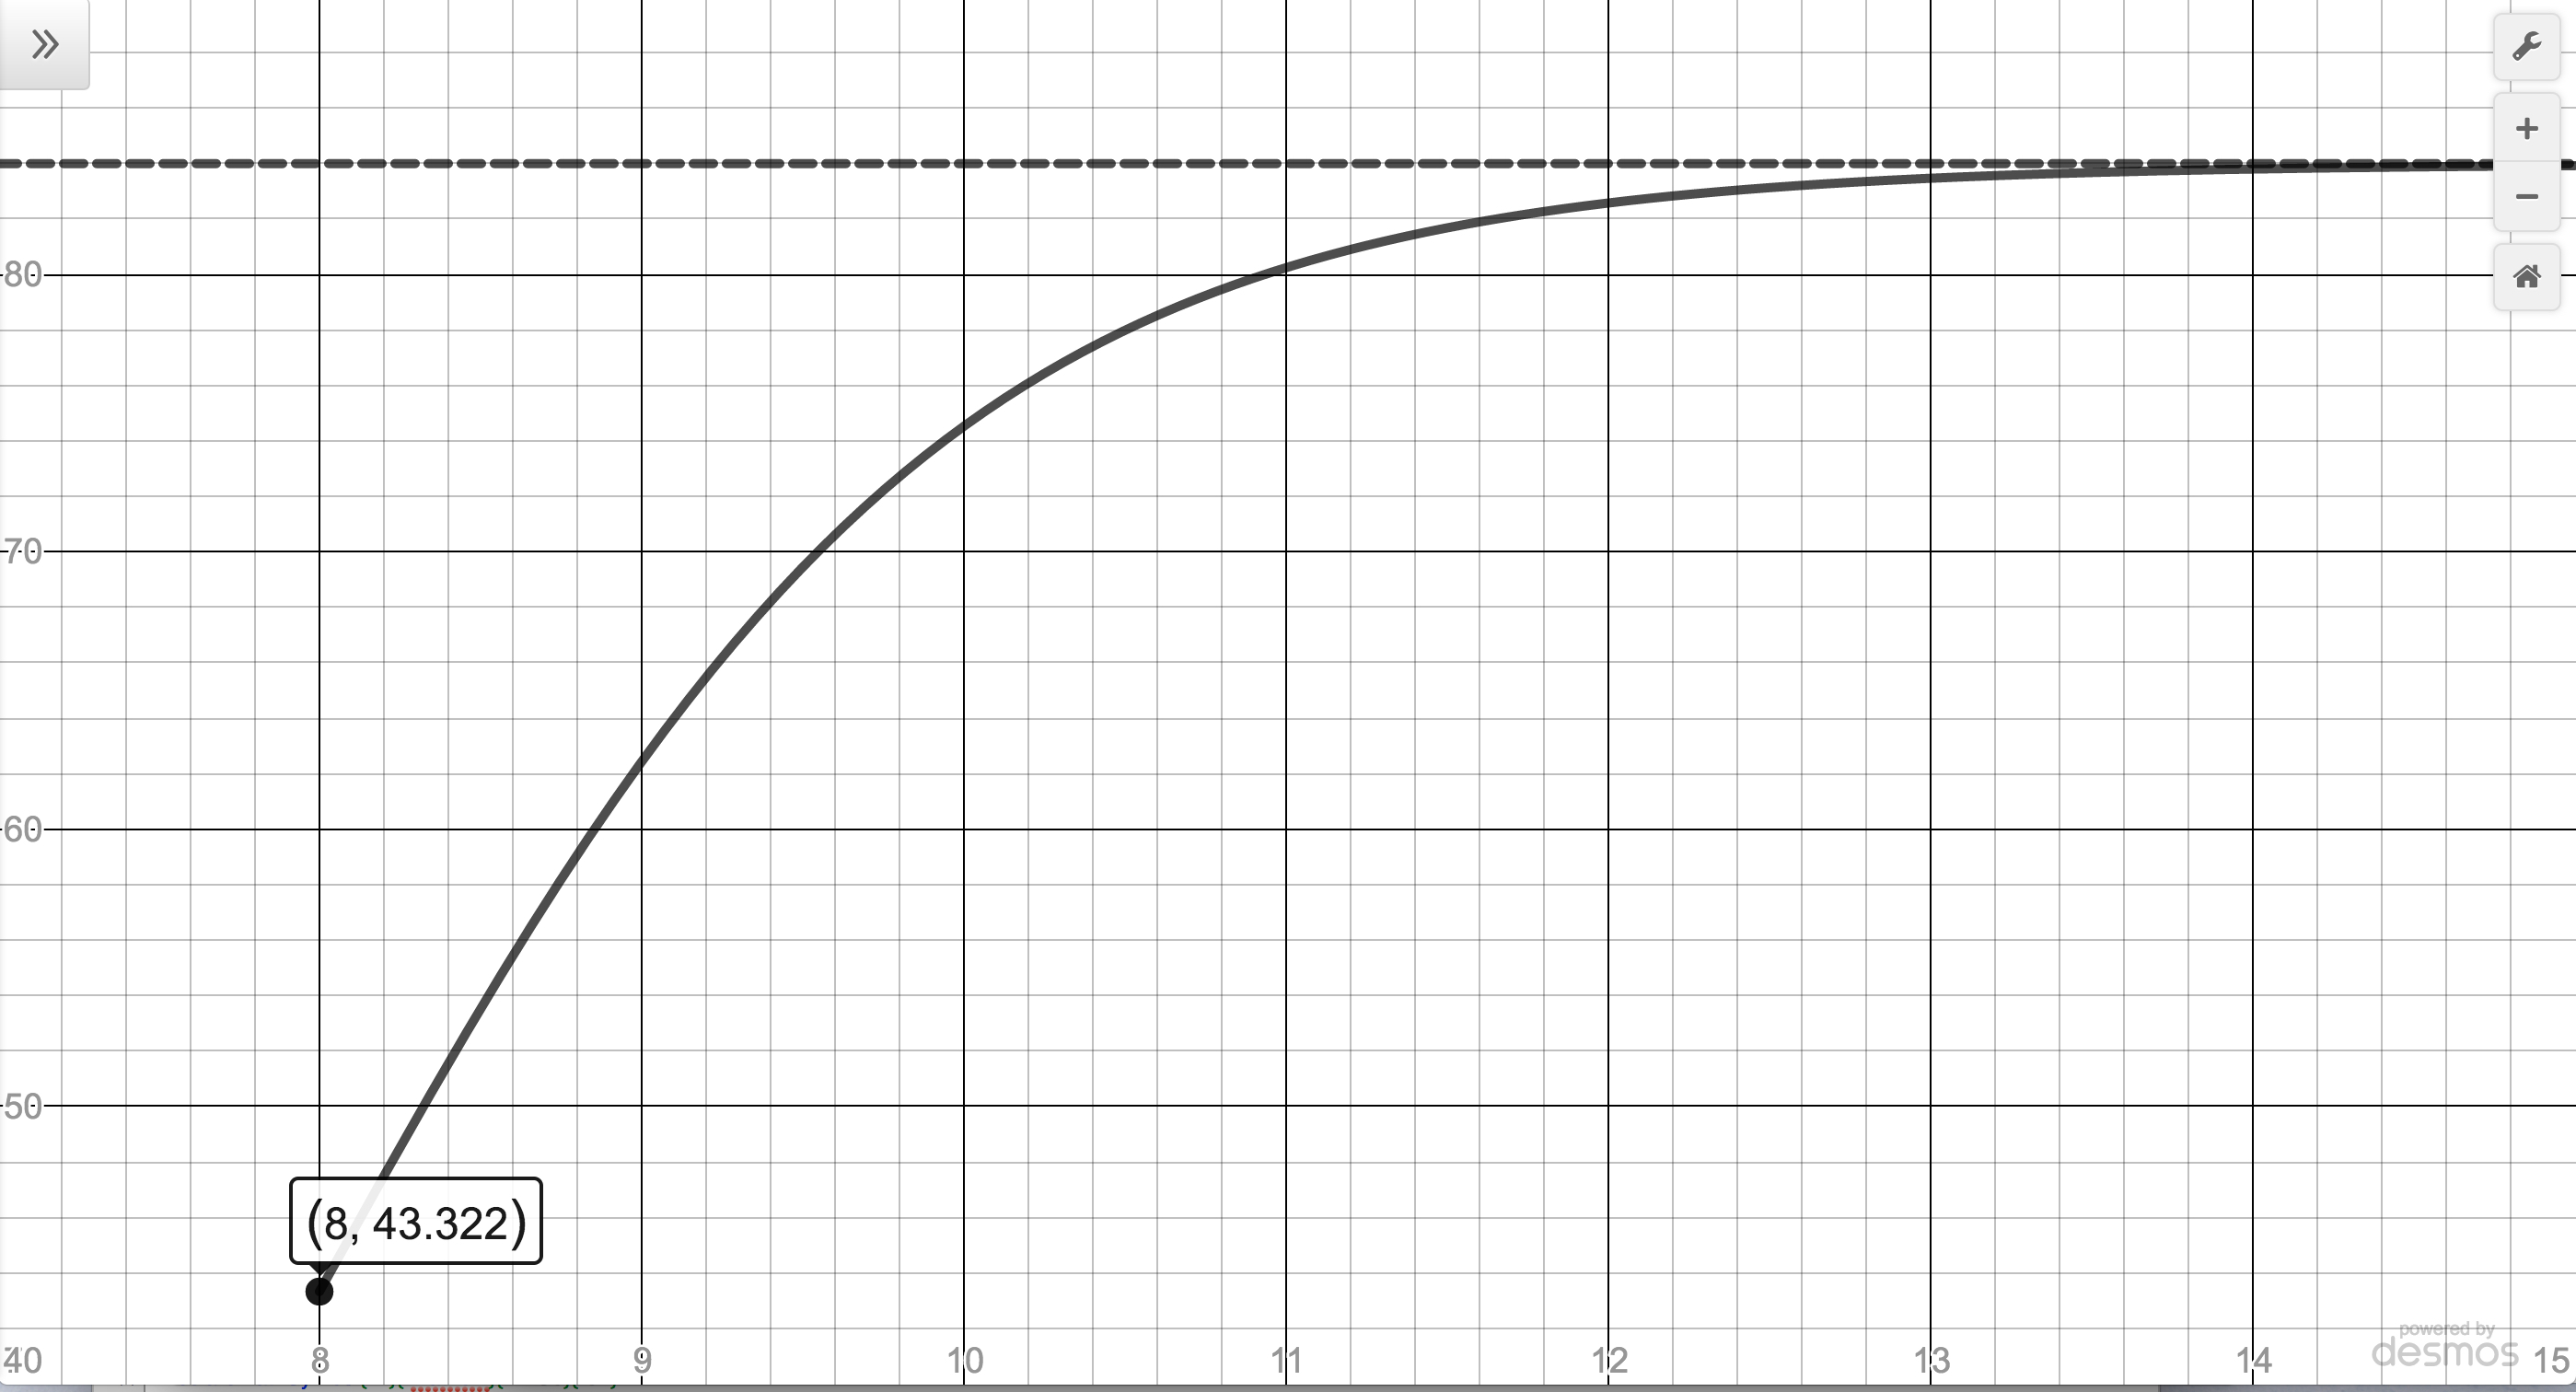
\includegraphics[width=3in]{./ApplicationsofExponentialandLogarithmicFunctionsGraphics/ExpLogAppEx03.jpg} \\

$y = N(t)$ for $0 \leq t \leq 8$ &

$y = N(t)$ for $8 \leq t \leq 15$

\end{tabular}

\end{center}


\subsection{Applications of Logarithms}

Just as many physical phenomena can be modeled by exponential functions, the same is true of logarithmic functions.   In Exercises \ref{Richterexercise},  \ref{decibelexercise} and \ref{pHexercise} of Section \ref{LogarithmicFunctions}, we showed that logarithms are useful in measuring the intensities of earthquakes (the Richter scale), sound (decibels) and acids and bases (pH).  We now present yet a different use of the a basic logarithm function, \href{http://en.wikipedia.org/wiki/Password_strength}{\underline{password strength}}.

\smallskip

\begin{ex}  The \href{http://en.wikipedia.org/wiki/Information_entropy}{\underline{information entropy}} $H$, in bits, of a randomly generated password consisting of $L$ characters is given by $H = L \log_{2}(N)$, where $N$ is the number of possible symbols for each character in the password.  In general, the higher the entropy, the stronger the password. \index{password strength} \index{information entropy}

\begin{enumerate}

\item  If a $7$ character case-sensitive\footnote{That is, upper and lower case letters are treated as different characters.} password is comprised of  letters and numbers only, find the associated information entropy.

\item  How many possible symbol options per character is required to produce a $7$ character password with an information entropy of $50$ bits?

\end{enumerate}

{\bf Solution.}

\begin{enumerate}

\item  There are $26$ letters in the alphabet, $52$ if upper and lower case letters are counted as different.  There are $10$ digits ($0$ through $9$) for a total of $N=62$ symbols.  Since the password is to be $7$ characters long, $L = 7$.  Thus, $H = 7 \log_{2}(62) = \frac{7 \ln(62)}{\ln(2)} \approx 41.68$.

\item  We have $L = 7$ and $H=50$ and we need to find $N$.  Solving the equation $50 = 7 \log_{2}(N)$ gives $N = 2^{50/7} \approx 141.323$, so we would need $142$ different symbols to choose from.\footnote{Since there are only $94$ distinct ASCII keyboard characters, to achieve this strength, the number of characters in the password should be increased.} \qed

\end{enumerate}

\end{ex}

\smallskip

Chemical systems known as \href{http://en.wikipedia.org/wiki/Buffer_solutions}{\underline{buffer solutions}} \index{buffer solution} have the ability to adjust to small changes in acidity to maintain a range of pH values.  Buffer solutions have a wide variety of applications from maintaining a healthy fish tank to regulating the pH levels in blood.  Our next example shows how the pH in a buffer solution is a little more complicated than the pH we first encountered in Exercise \ref{pHexercise} in Section \ref{LogarithmicFunctions}. 

\smallskip

\begin{ex}  Blood is a buffer solution. When carbon dioxide is absorbed into the bloodstream it produces carbonic acid and lowers the pH.  The body compensates by producing bicarbonate, a weak base to partially neutralize the acid.   The equation\footnote{Derived from the \href{http://en.wikipedia.org/wiki/Henderson-Hasselbalch_equation}{\underline{Henderson-Hasselbalch Equation}}. See Exercise \ref{HendersonHasselbalch} in Section \ref{PropertiesofLogarithms}.  Hasselbalch himself was studying carbon dioxide dissolving in blood - a process called \href{http://en.wikipedia.org/wiki/Metabolic_acidosis}{\underline{metabolic acidosis}}.}   which models blood pH in this situation is $\mbox{pH} = 6.1 + \log\left(\frac{800}{x} \right)$, where $x$ is the partial pressure of carbon dioxide in arterial blood, measured in torr. Find the partial pressure of carbon dioxide in arterial blood if the pH is $7.4$.

\smallskip

{\bf Solution.}  We set $\mbox{pH} = 7.4$ and get $ 7.4 = 6.1 + \log\left(\frac{800}{x} \right)$, or $\log\left(\frac{800}{x} \right) = 1.3$.   We get $x = \frac{800}{10^{1.3}} \approx 40.09$.  Hence, the partial pressure of carbon dioxide in the blood is about $40$ torr. \qed


\end{ex}

Another place logarithms are used is in data analysis. Suppose, for instance, we wish to model the spread of influenza A (H1N1), the so-called `Swine Flu'.  Below is data taken from the World Health Organization (\href{http://www.who.int/csr/disease/swineflu/updates/en/index.html}{\underline{WHO}}) where $t$ represents the number of days since April 28, 2009, and $N$ represents the number of confirmed cases of H1N1 virus worldwide.

\[ \begin{array}{|c||c|c|c|c|c|c|c|c|c|c|c|c|c|}  \hline

t & 1 & 2 & 3 & 4 & 5 & 6 & 7 & 8 & 9 & 10 & 11 & 12 & 13  \\ \hline

N & 148 & 257 &   367 & 658 & 898 & 1085 & 1490 & 1893 & 2371 & 2500 & 3440 & 4379 & 4694  \\ \hline \end{array} \]


\[\begin{array}{|c||c||c|c|c|c|c|c|} \hline

t & 14 & 15 & 16 & 17 & 18 & 19& 20  \\ \hline 

N & 5251 & 5728 & 6497 & 7520 & 8451 & 8480 & 8829    \\ \hline \end{array} \]

Making a scatter plot of the data treating $t$ as the independent variable and $N$ as the dependent variable gives the plot below on the left.  Which models are suggested by the shape of the data?  

\smallskip

Thinking back Section \ref{QuadraticFunctions}, we try a Quadratic Regression.  We find $N(t) \approx 16.713 t^2 +149.68t -233.15$ with $R^2 = 0.992$, indicating a pretty good fit.  However, is there any underlying scientific principle which would account for these data to be quadratic?  Are there other models which fit the data  better?


\begin{center}

\begin{tabular}{cc}

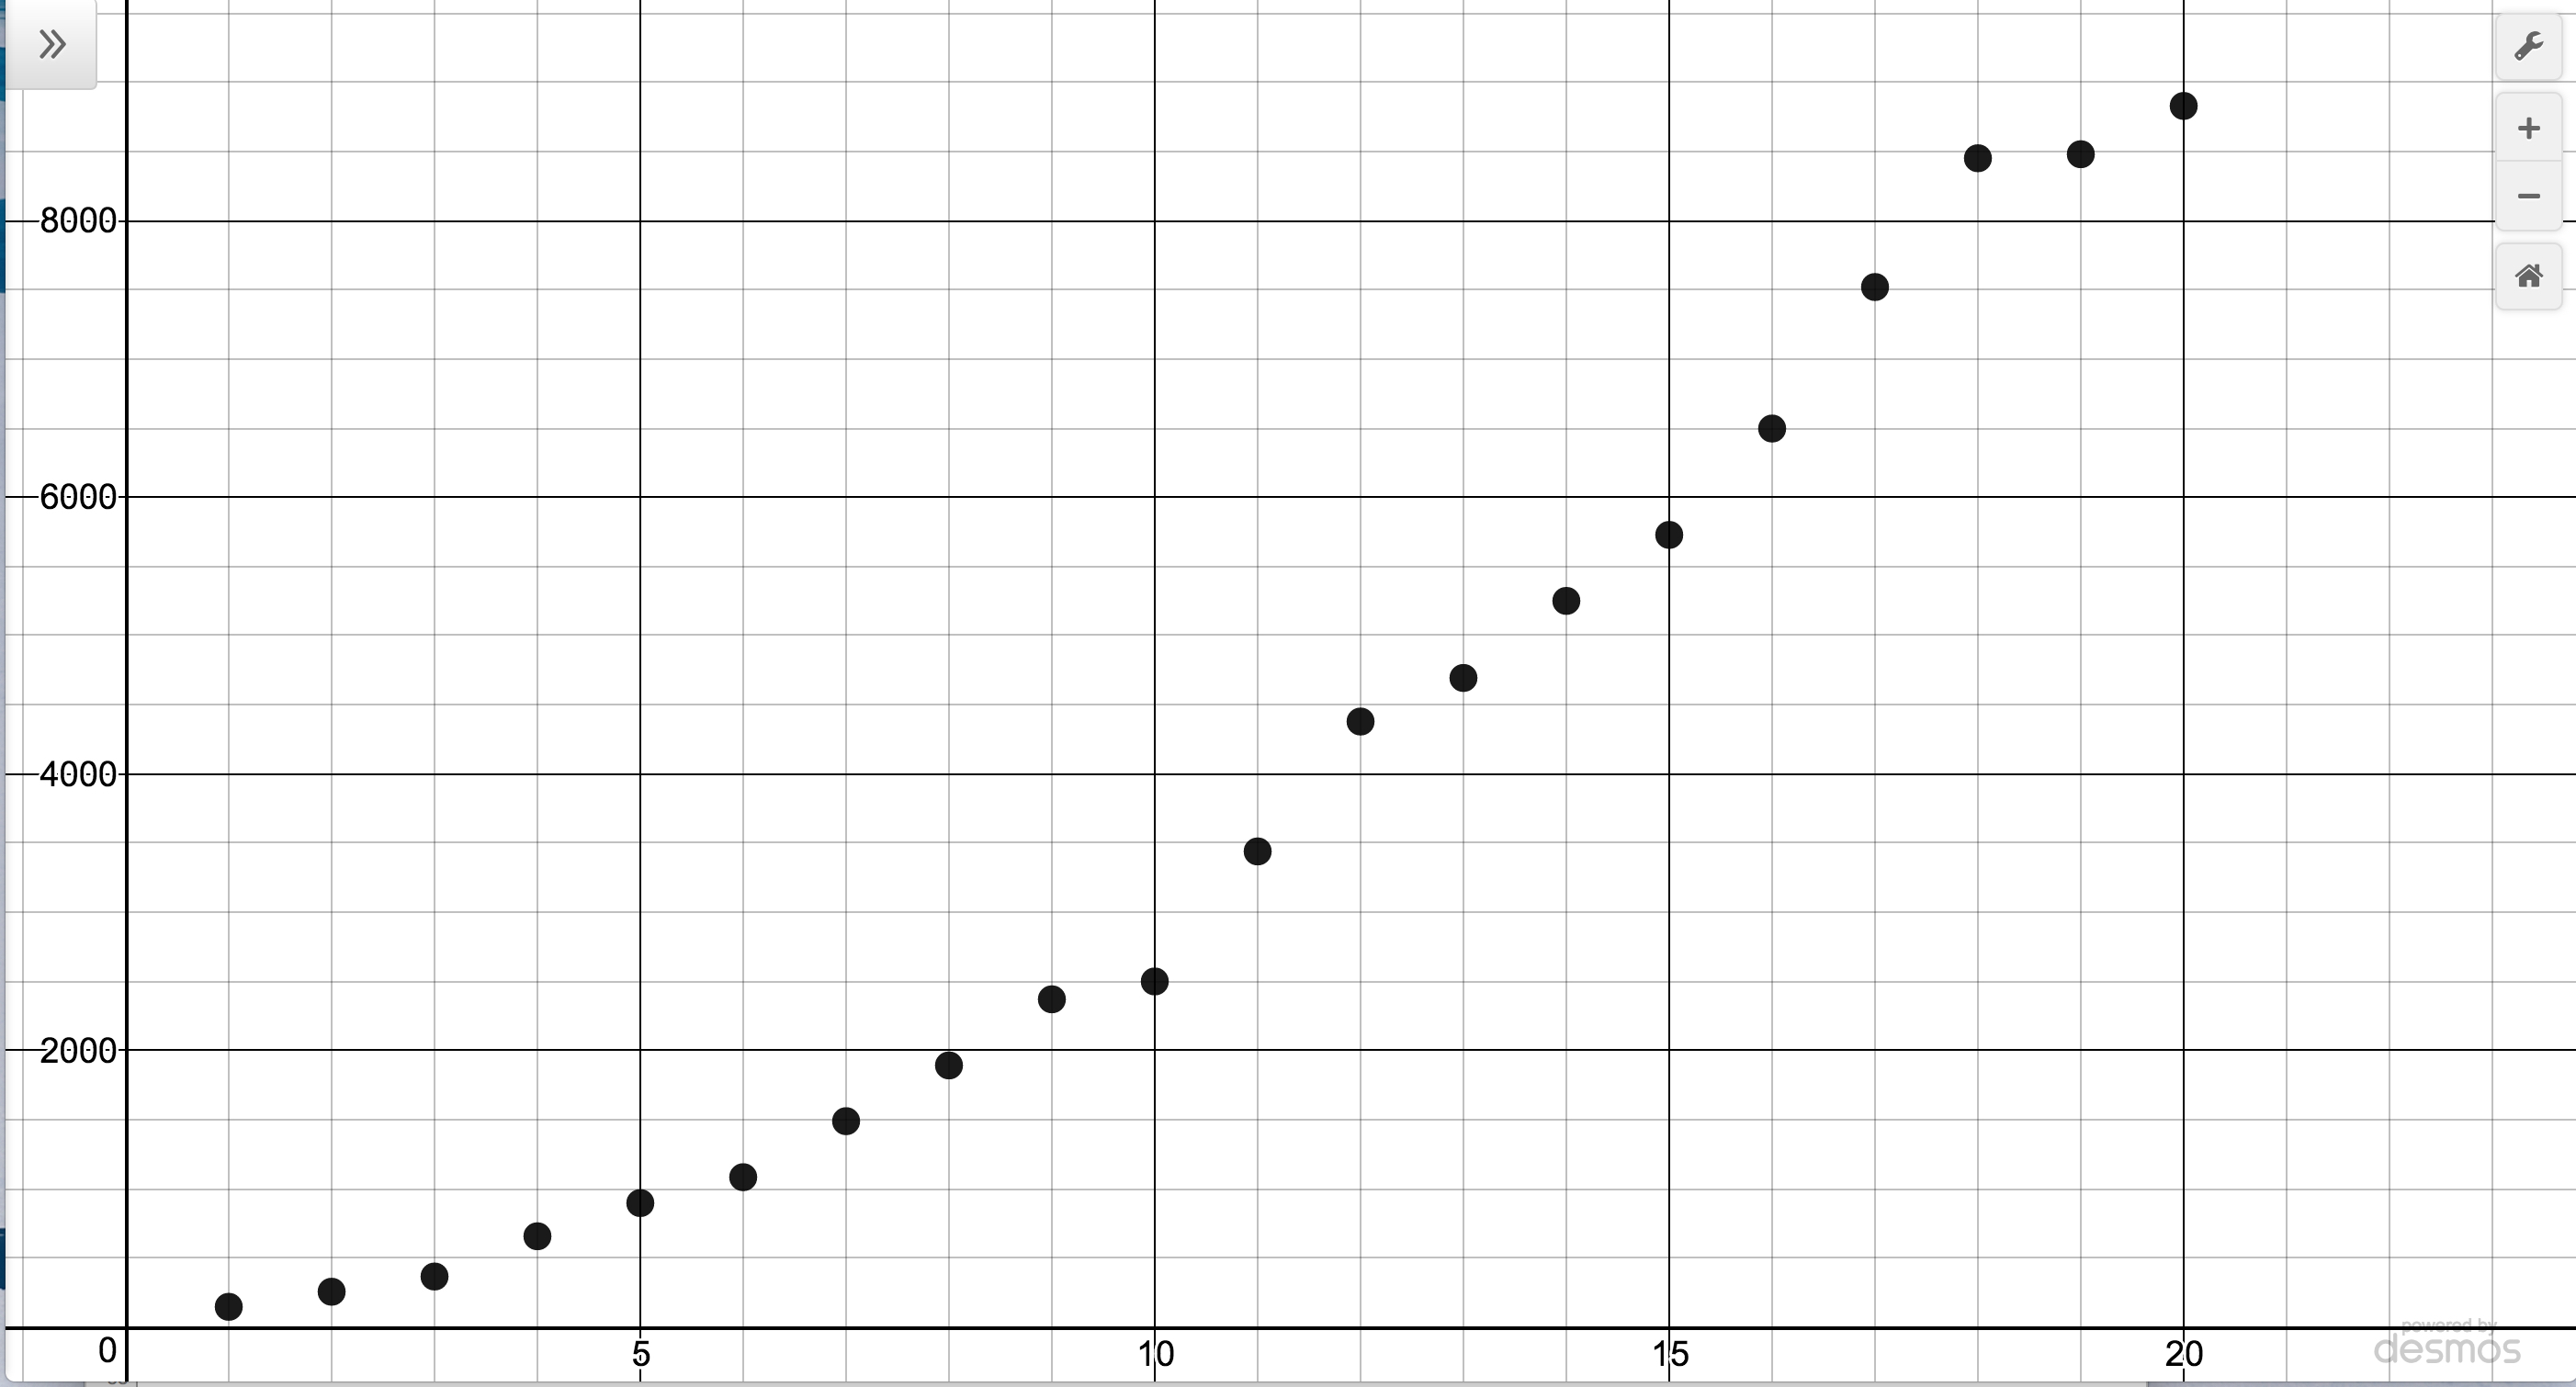
\includegraphics[width=3in]{./ApplicationsofExponentialandLogarithmicFunctionsGraphics/ExpLogAppEx04.jpg} &

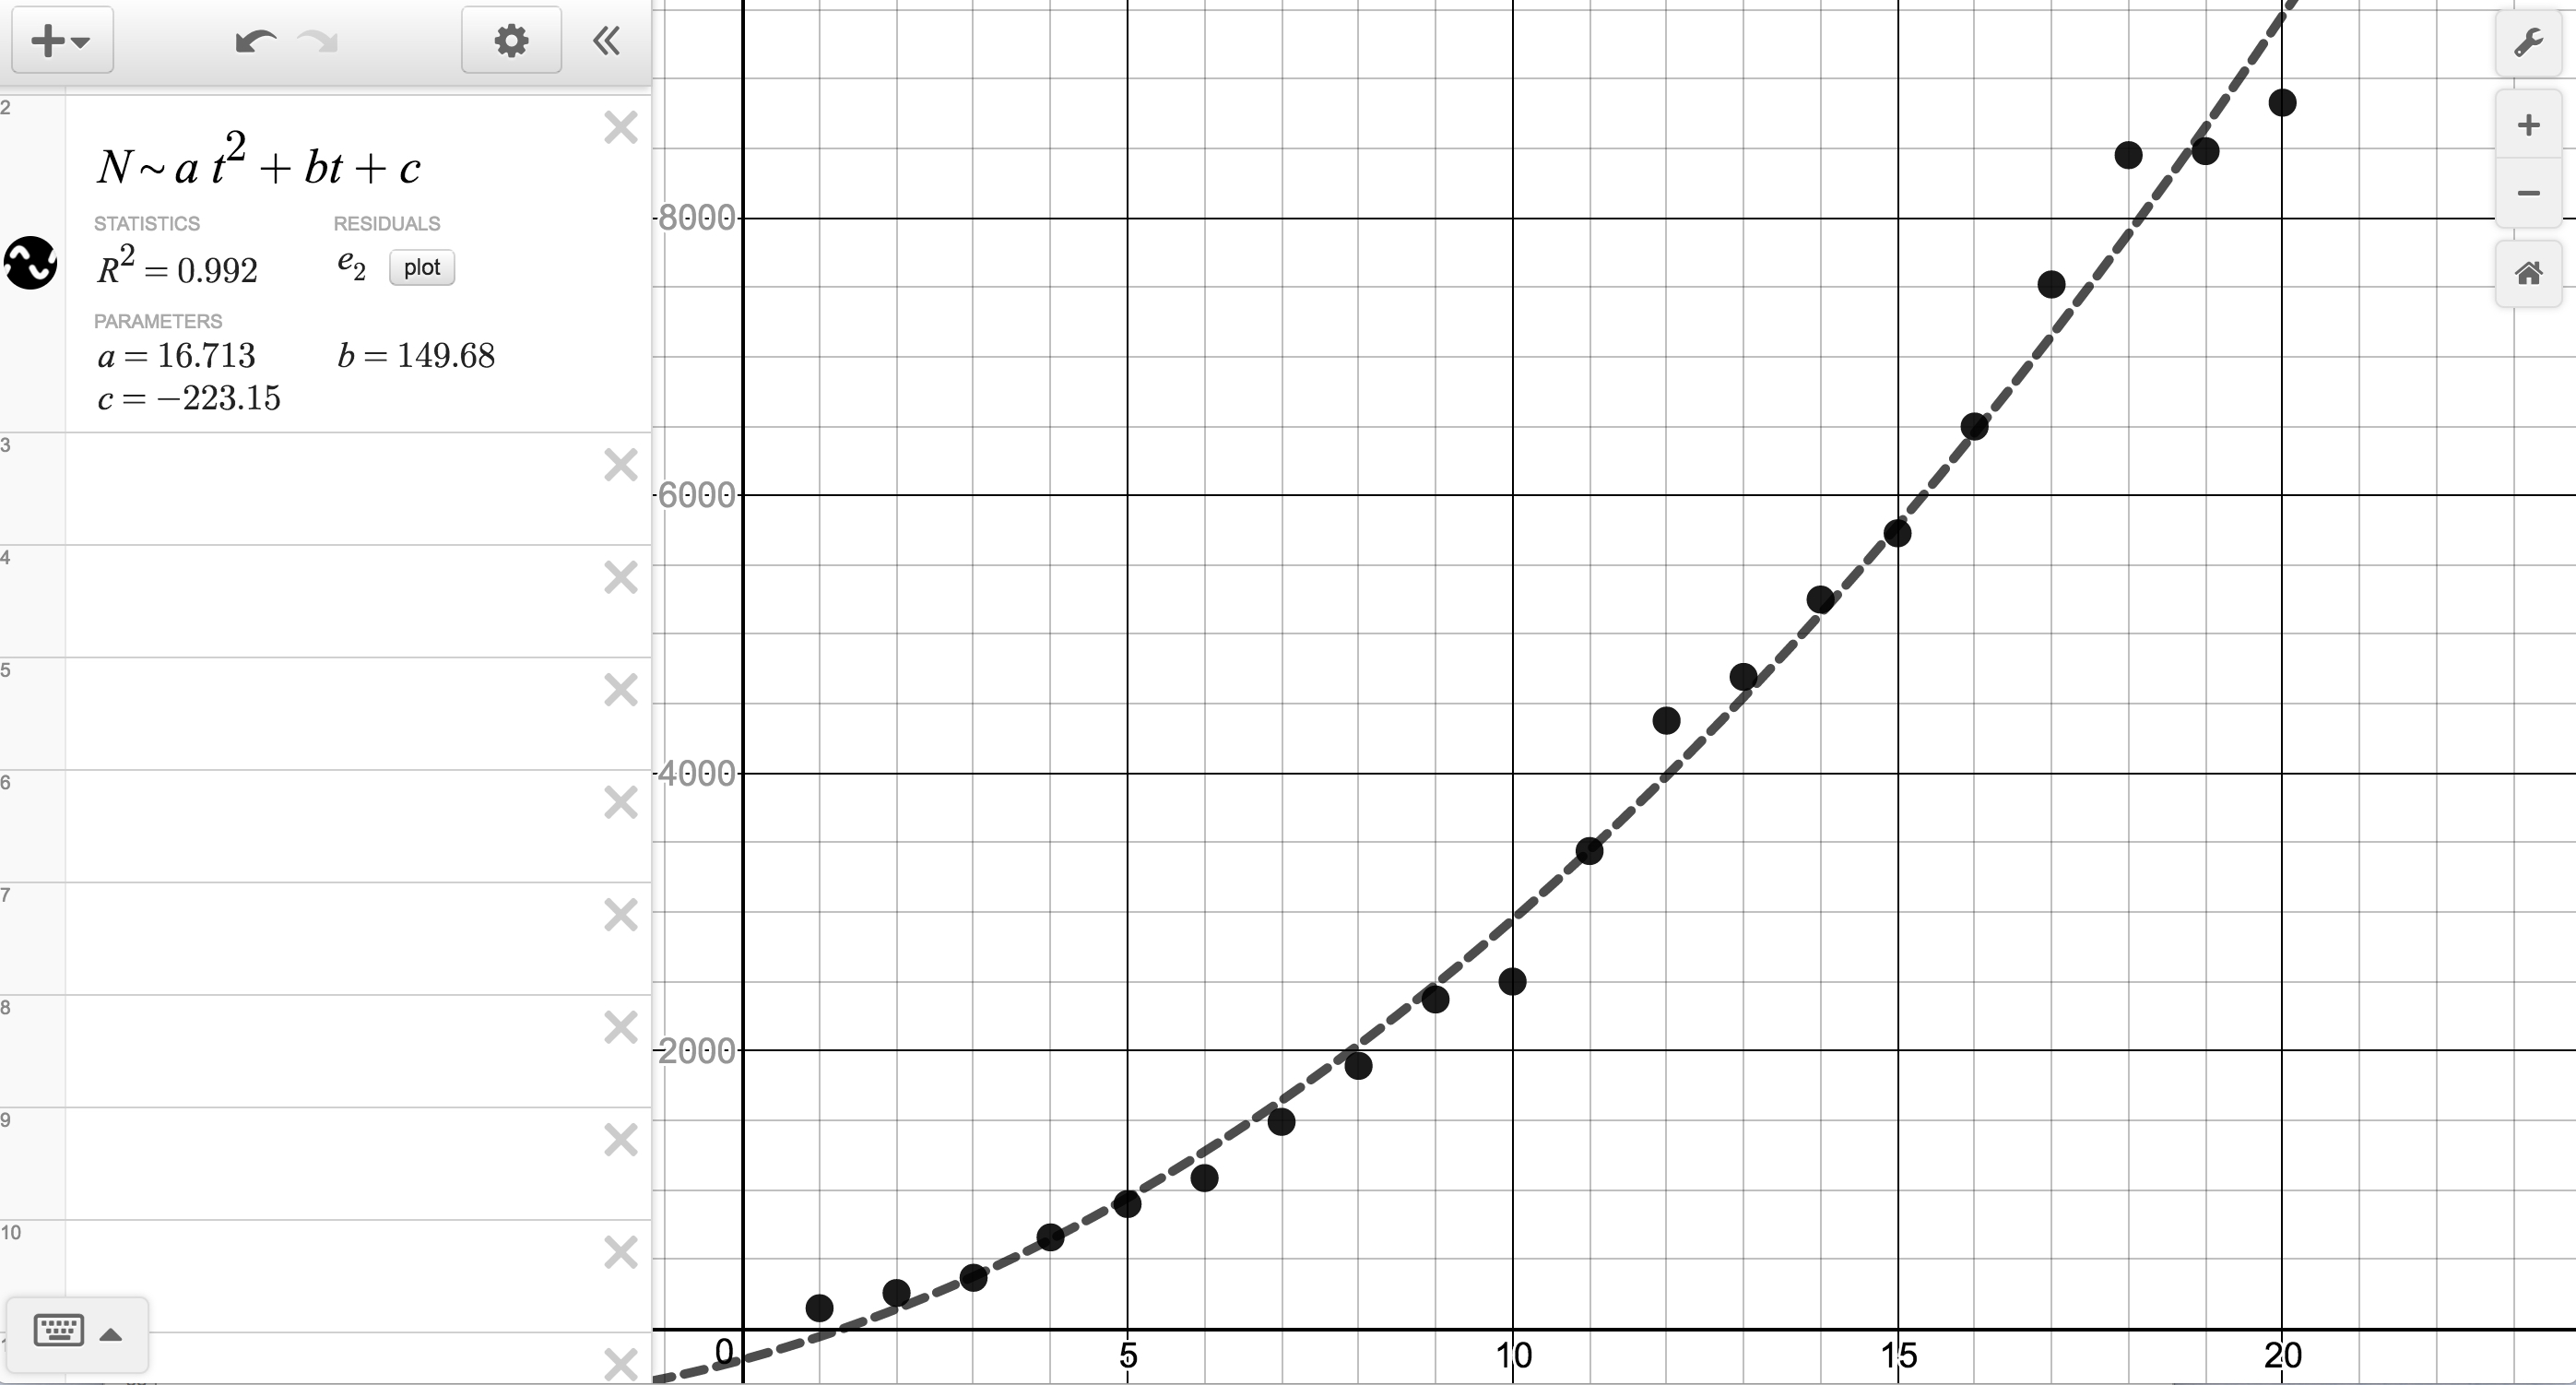
\includegraphics[width=3in]{./ApplicationsofExponentialandLogarithmicFunctionsGraphics/ExpLogAppEx05.jpg} \\

Scatterplot of the Data &

A quadratic regression model \\

\end{tabular}

\end{center}

To answer these questions, scientists often use logarithms in an attempt to `linearize' non-liner data sets such as the one before us.  To see how this could work, suppose we guessed the relationship between $N$ and $t$ is something from Section \ref{PowerFunctions},  $N(t) = a t^{p}$.  

\smallskip

By taking the natural logs of both sides and using the Product and Power Rules, in turn, we find that $\ln(N(t)) = \ln(a t^p) = \ln(a) + \ln(t^p) = \ln(a) + p \ln(t) =  p \ln(t) + \ln(a)$.   If we let  $x = \ln(t)$ and $y= \ln(N(t))$,  the model takes the form $y = p x + \ln(a)$ which is a \textit{linear} model with slope $p$ and $y$-intercept $\ln(a)$.  So, instead of plotting $N(t)$ versus $t$, we plot $y=\ln(N(t))$ versus $x=\ln(t)$ and find a linear regression for this data set.

\[ \begin{array}{|c||c|c|c|c|c|c|c|c|c|c|c|c|c|}  \hline

\ln(t) & 0 & 0.693 & 1.099 & 1.386& 1.609 & 1.792 & 1.946 & 2.079 & 2.197 & 2.302 & 2.398 & 2.485 & 2.565  \\ \hline

\ln(N) & 4.997  & 5.549 &  5.905 & 6.489 & 6.800 & 6.989 & 7.306 & 7.546 & 7.771 & 7.824 & 8.143 & 8.385 & 8.454  \\ \hline \end{array} \]


\[\begin{array}{|c||c||c|c|c|c|c|c|} \hline

\ln(t) & 2.639 & 2.708 & 2.773 & 2.833 & 2.890 & 2.944 & 2.996  \\ \hline 

\ln(N) & 8.566 & 8.653 & 8.779 & 8.925 & 9.042 & 9.045 & 9.086    \\ \hline \end{array} \]

\begin{center}

\begin{tabular}{cc}

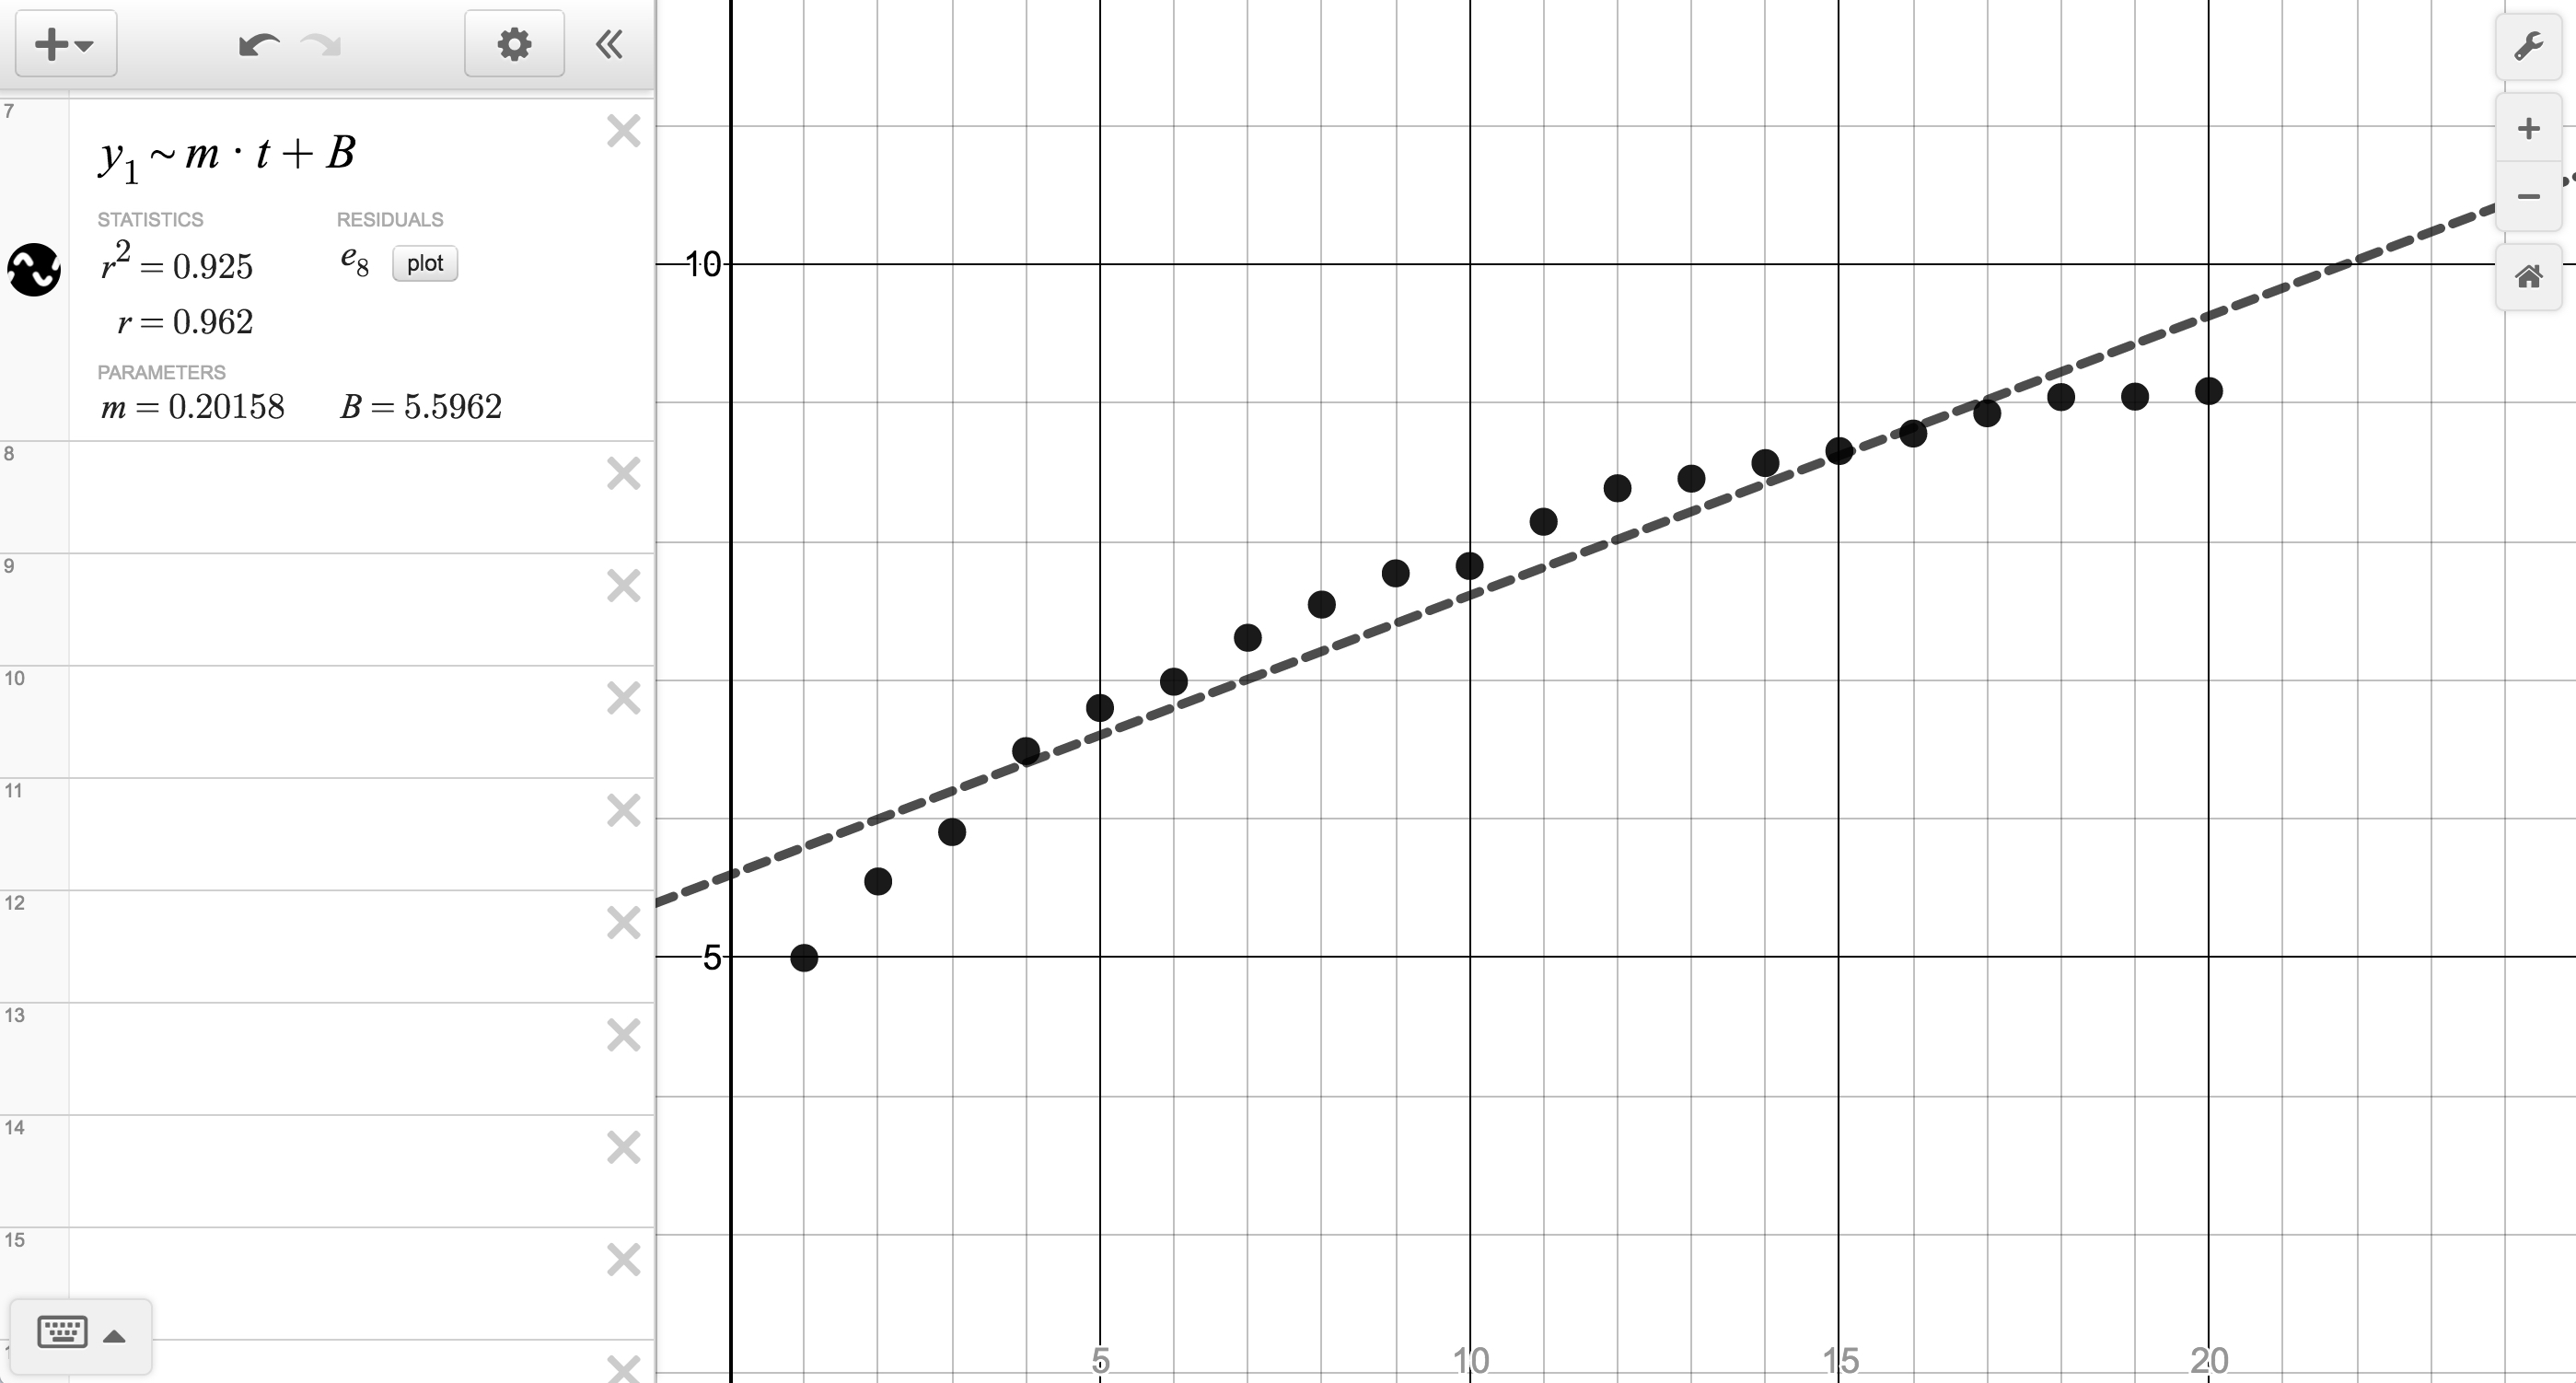
\includegraphics[width=3in]{./ApplicationsofExponentialandLogarithmicFunctionsGraphics/ExpLogAppEx10.jpg} &

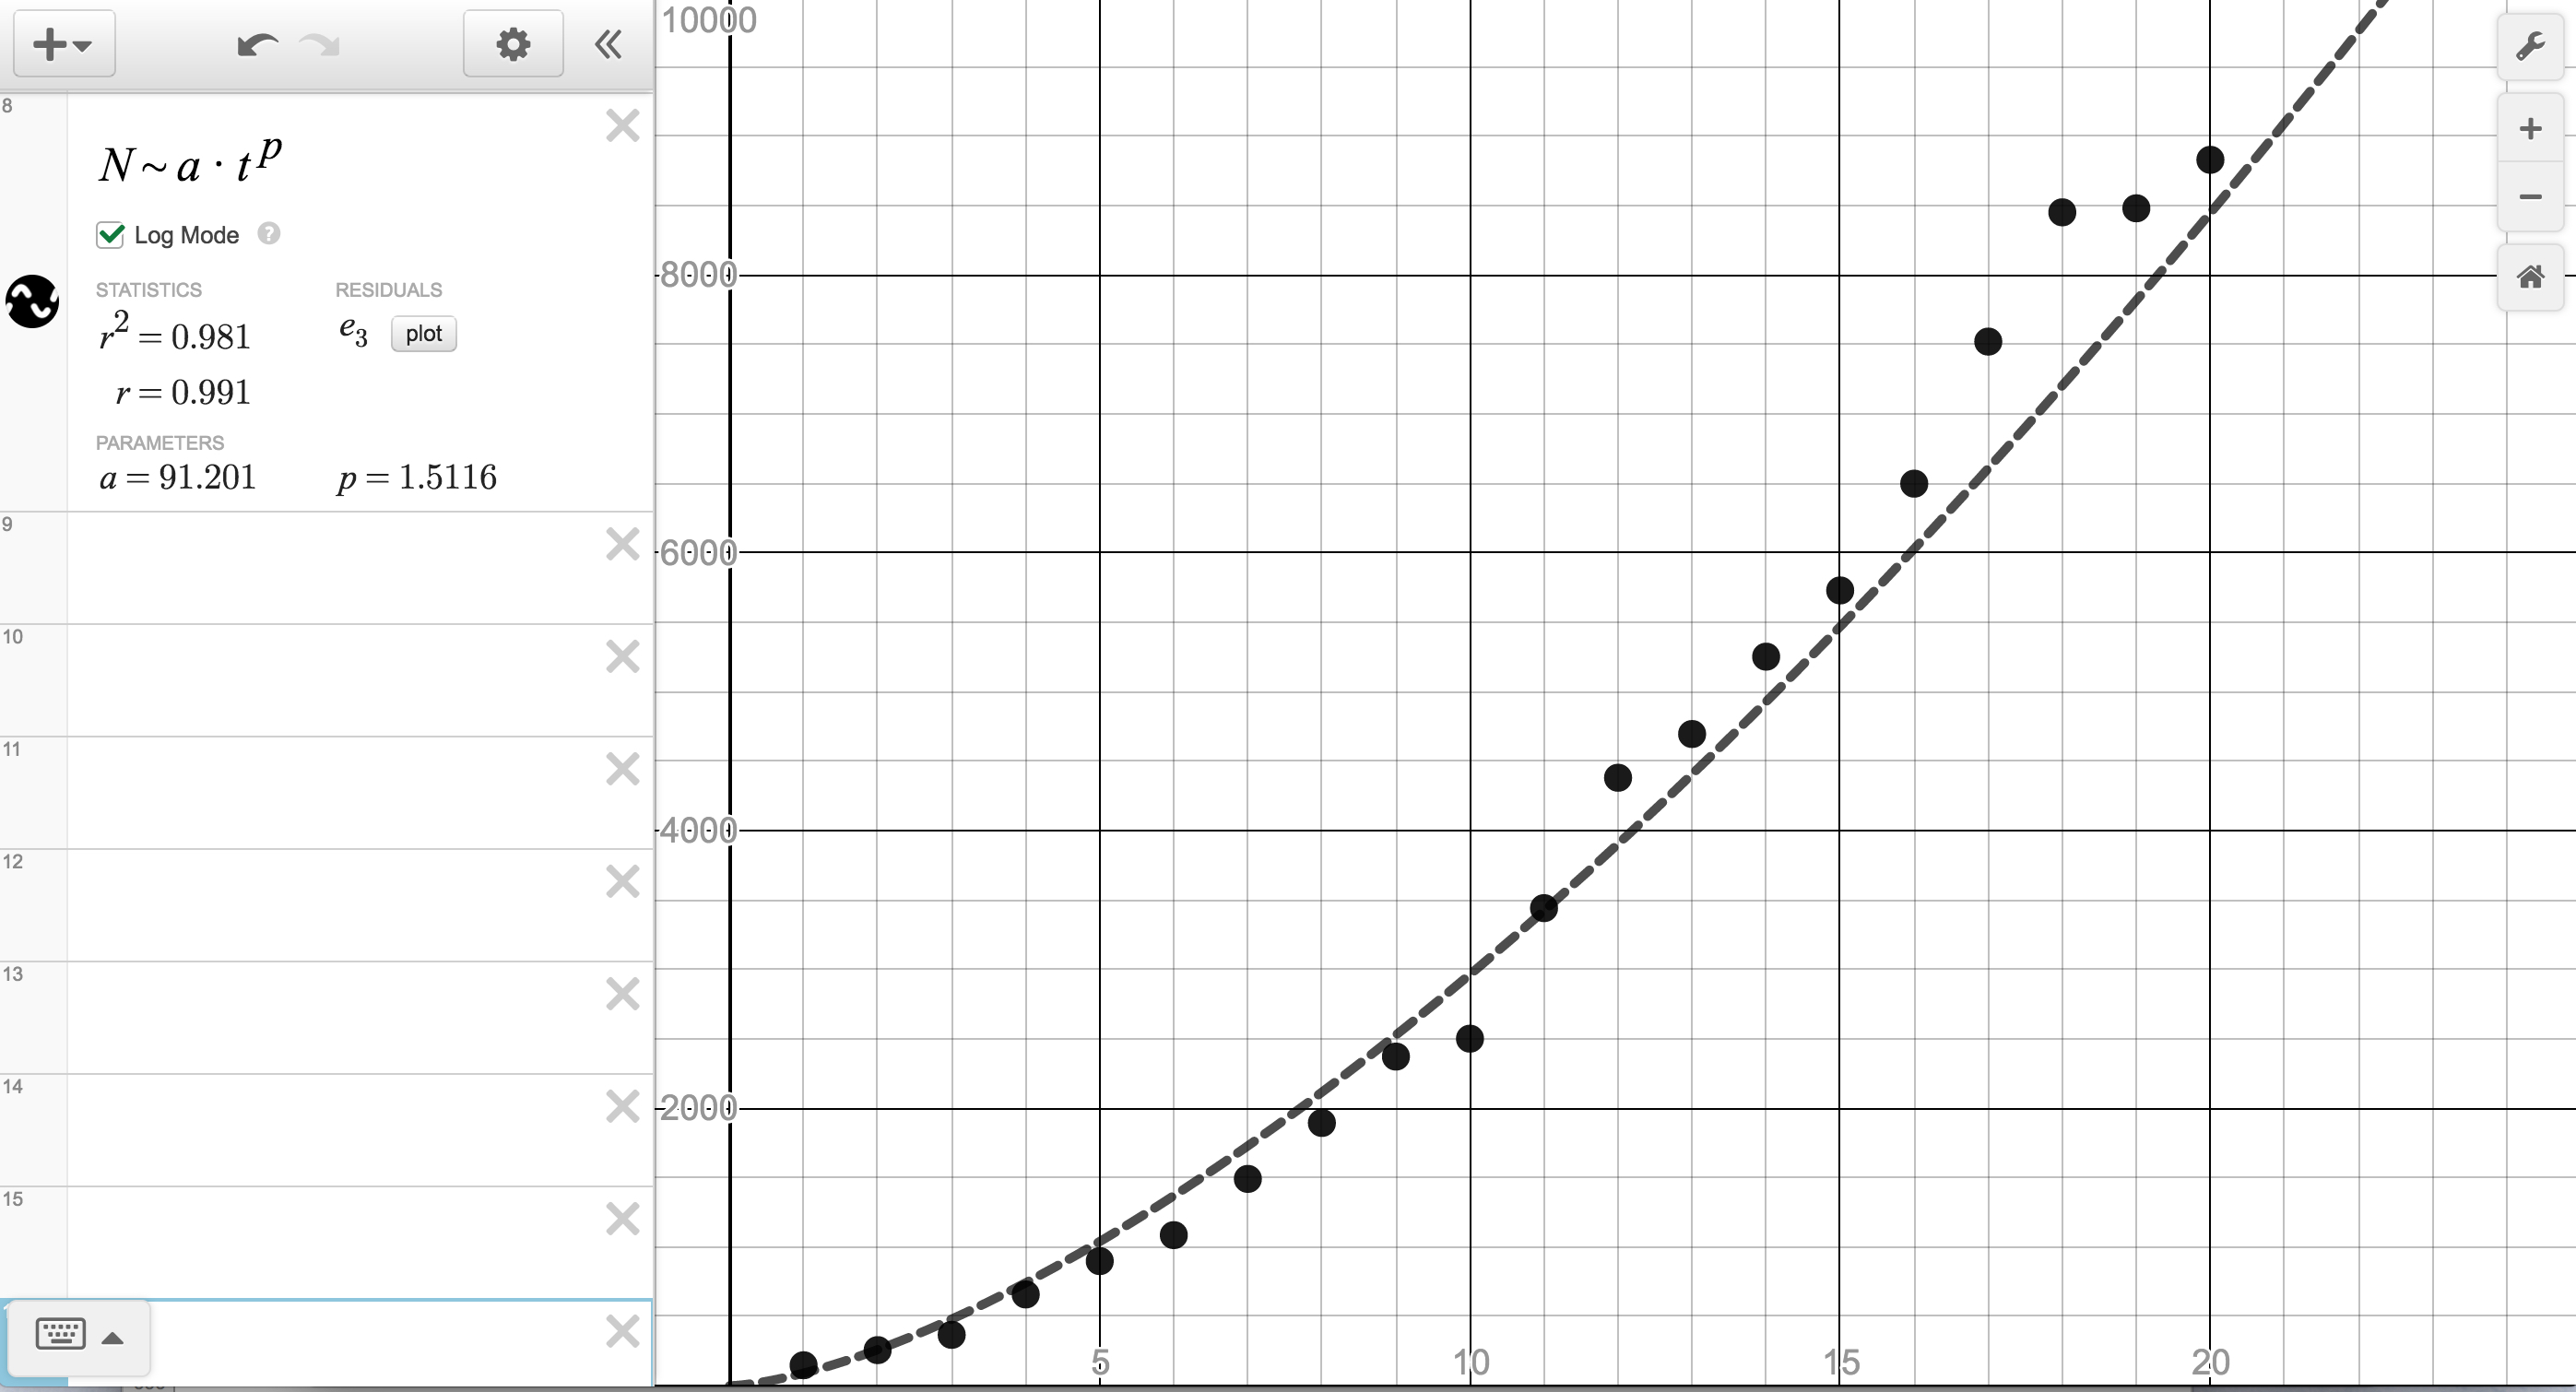
\includegraphics[width=3in]{./ApplicationsofExponentialandLogarithmicFunctionsGraphics/ExpLogAppEx06a.jpg} \\

linear regression: $\ln(N(t)) = p \ln(t) + \ln(a)$ &

power function regression: $N(t) = at^{p}$ \\

\end{tabular}

\end{center}



We see $r=0.991$, which is very close to $1$ indicating a very good fit.   The slope of the regression line is $m \approx 1.512$ which corresponds to our exponent $p$.  The $y$-intercept $b \approx 4.513$ corresponds to $\ln(a)$, so that $a \approx 91.201$.  Hence, we get the model $N = 91.201 t^{1.512}$. 

\smallskip

Of interest here is that the graphing utility we used, \href{https://www.desmos.com}{\underline{desmos}} has its own built-in power regression model.  If the `log mode'  square is checked, the graphing utility returns the \textit{same} model we obtained using our linearization (since the routine which determines the coefficients uses logarithms as well.)\footnote{If, however, we uncheck that box, we get a \textit{different} power function model, $N(t) = 62.318 t^{1.675}$ which chooses $a$ and $p$ directly to minimize the total squared error.  See \href{http://support.desmos.com/hc/en-us/articles/204349605}{\underline{here}} for more details.}

\smallskip

At this point, the quadratic model fits the data better, ostensibly because we have \textit{three} parameters we can adjust in the formula $N(t) = at^2+bt+c$ to minimize our error as opposed to just \textit{two} parameters in the formula $N(t) = a t^{p}$.  Neither  model, however, is based on any underlying scientific principle.

\smallskip

If we think about this situation from a scientific perspective, it does seem to make sense that, at least in the early stages of the outbreak, the more people who have the flu, the faster it will spread.  This suggests we fit the data to an uninhibited growth model.

\smallskip

As  written,  Equation \ref{lawofuninhibitedgrowth} gives uninhibited growth as  $N(t) = N_{\mbox{\tiny$0$}}e^{kt}$. Here, for simplicity's sake, we relabel $N_{\mbox{\tiny$0$}} = a$ and $e^{k} = b$ so that we are looking for parameters $a$ and $b$ so that $N(t) = a \cdot b^{t}$.

\smallskip

\phantomsection
\label{swineflulinearized}
If we assume $N(t) = a \cdot b^{t}$ then, taking logs as before, we get $\ln(N(t)) = t \ln(b) + \ln(a)$. If we let $y= \ln(N(t))$, then, once again, we get a linear model this time with slope $\ln(b)$ and $y$-intercept $\ln(a)$.  We present the results of the regression below.  While there is a strong correlation, $r = 0.962$, the plot doesn't instill the greatest of confidence in this model.

\begin{center}

\begin{tabular}{cc}

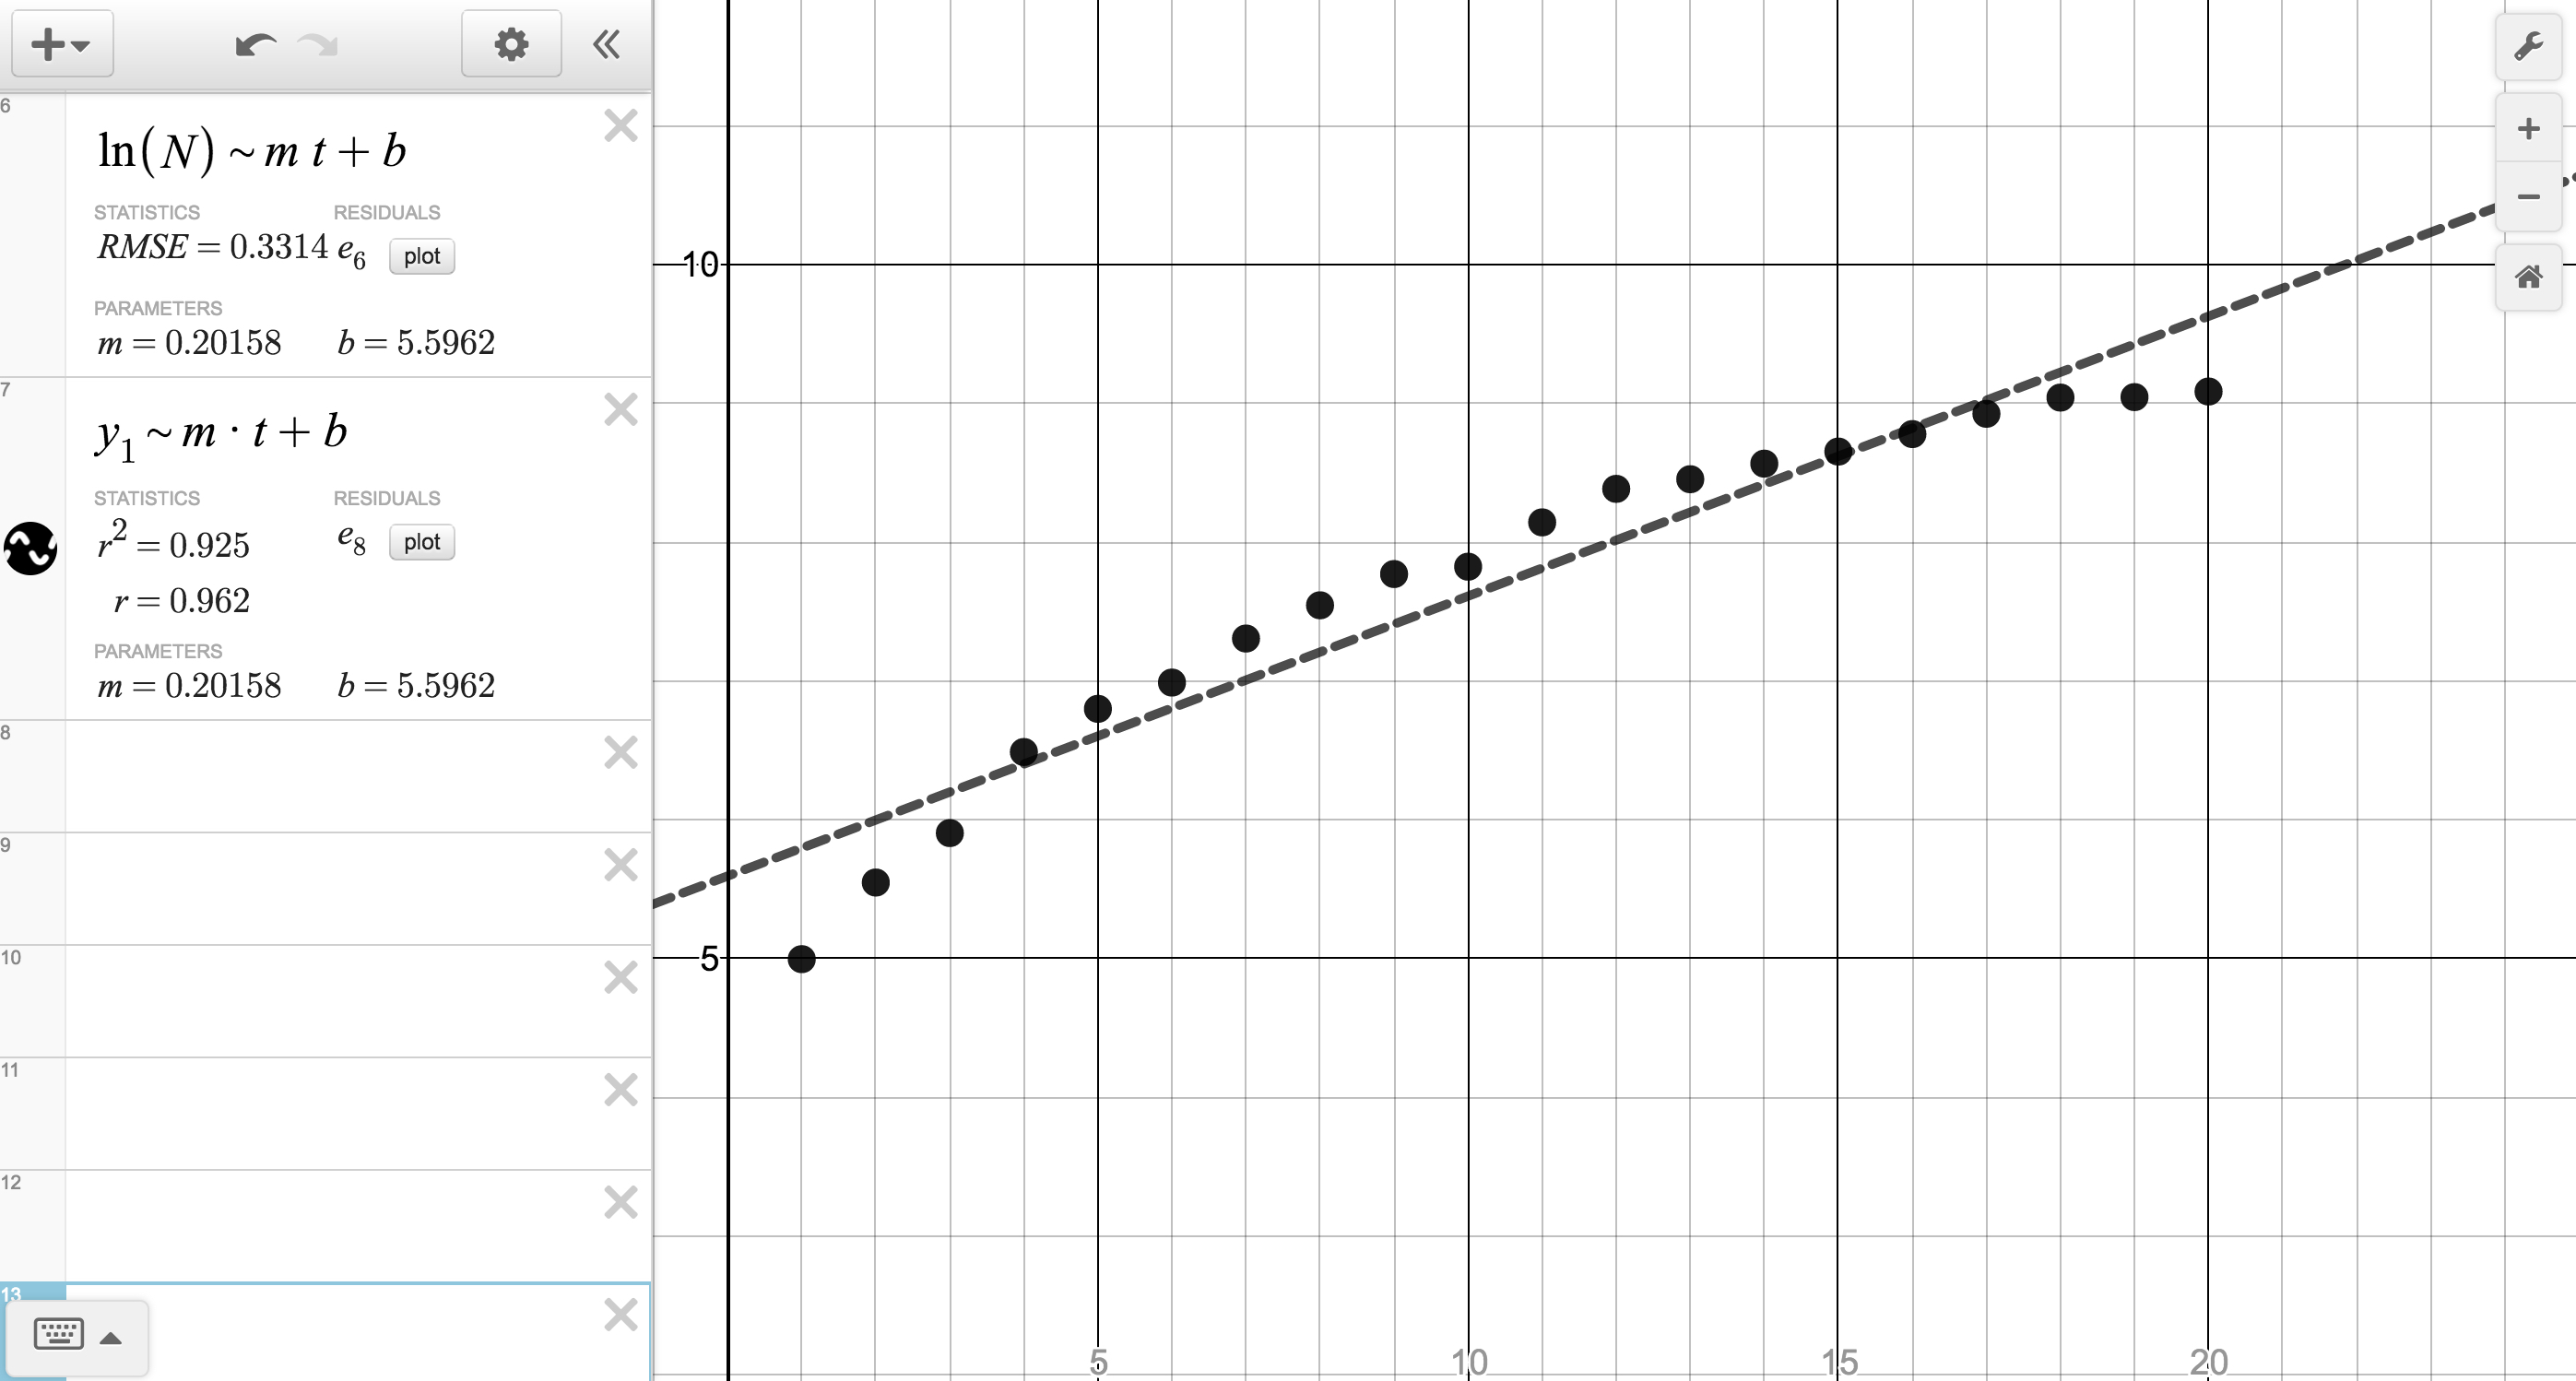
\includegraphics[width=3in]{./ApplicationsofExponentialandLogarithmicFunctionsGraphics/ExpLogAppEx09.jpg} &

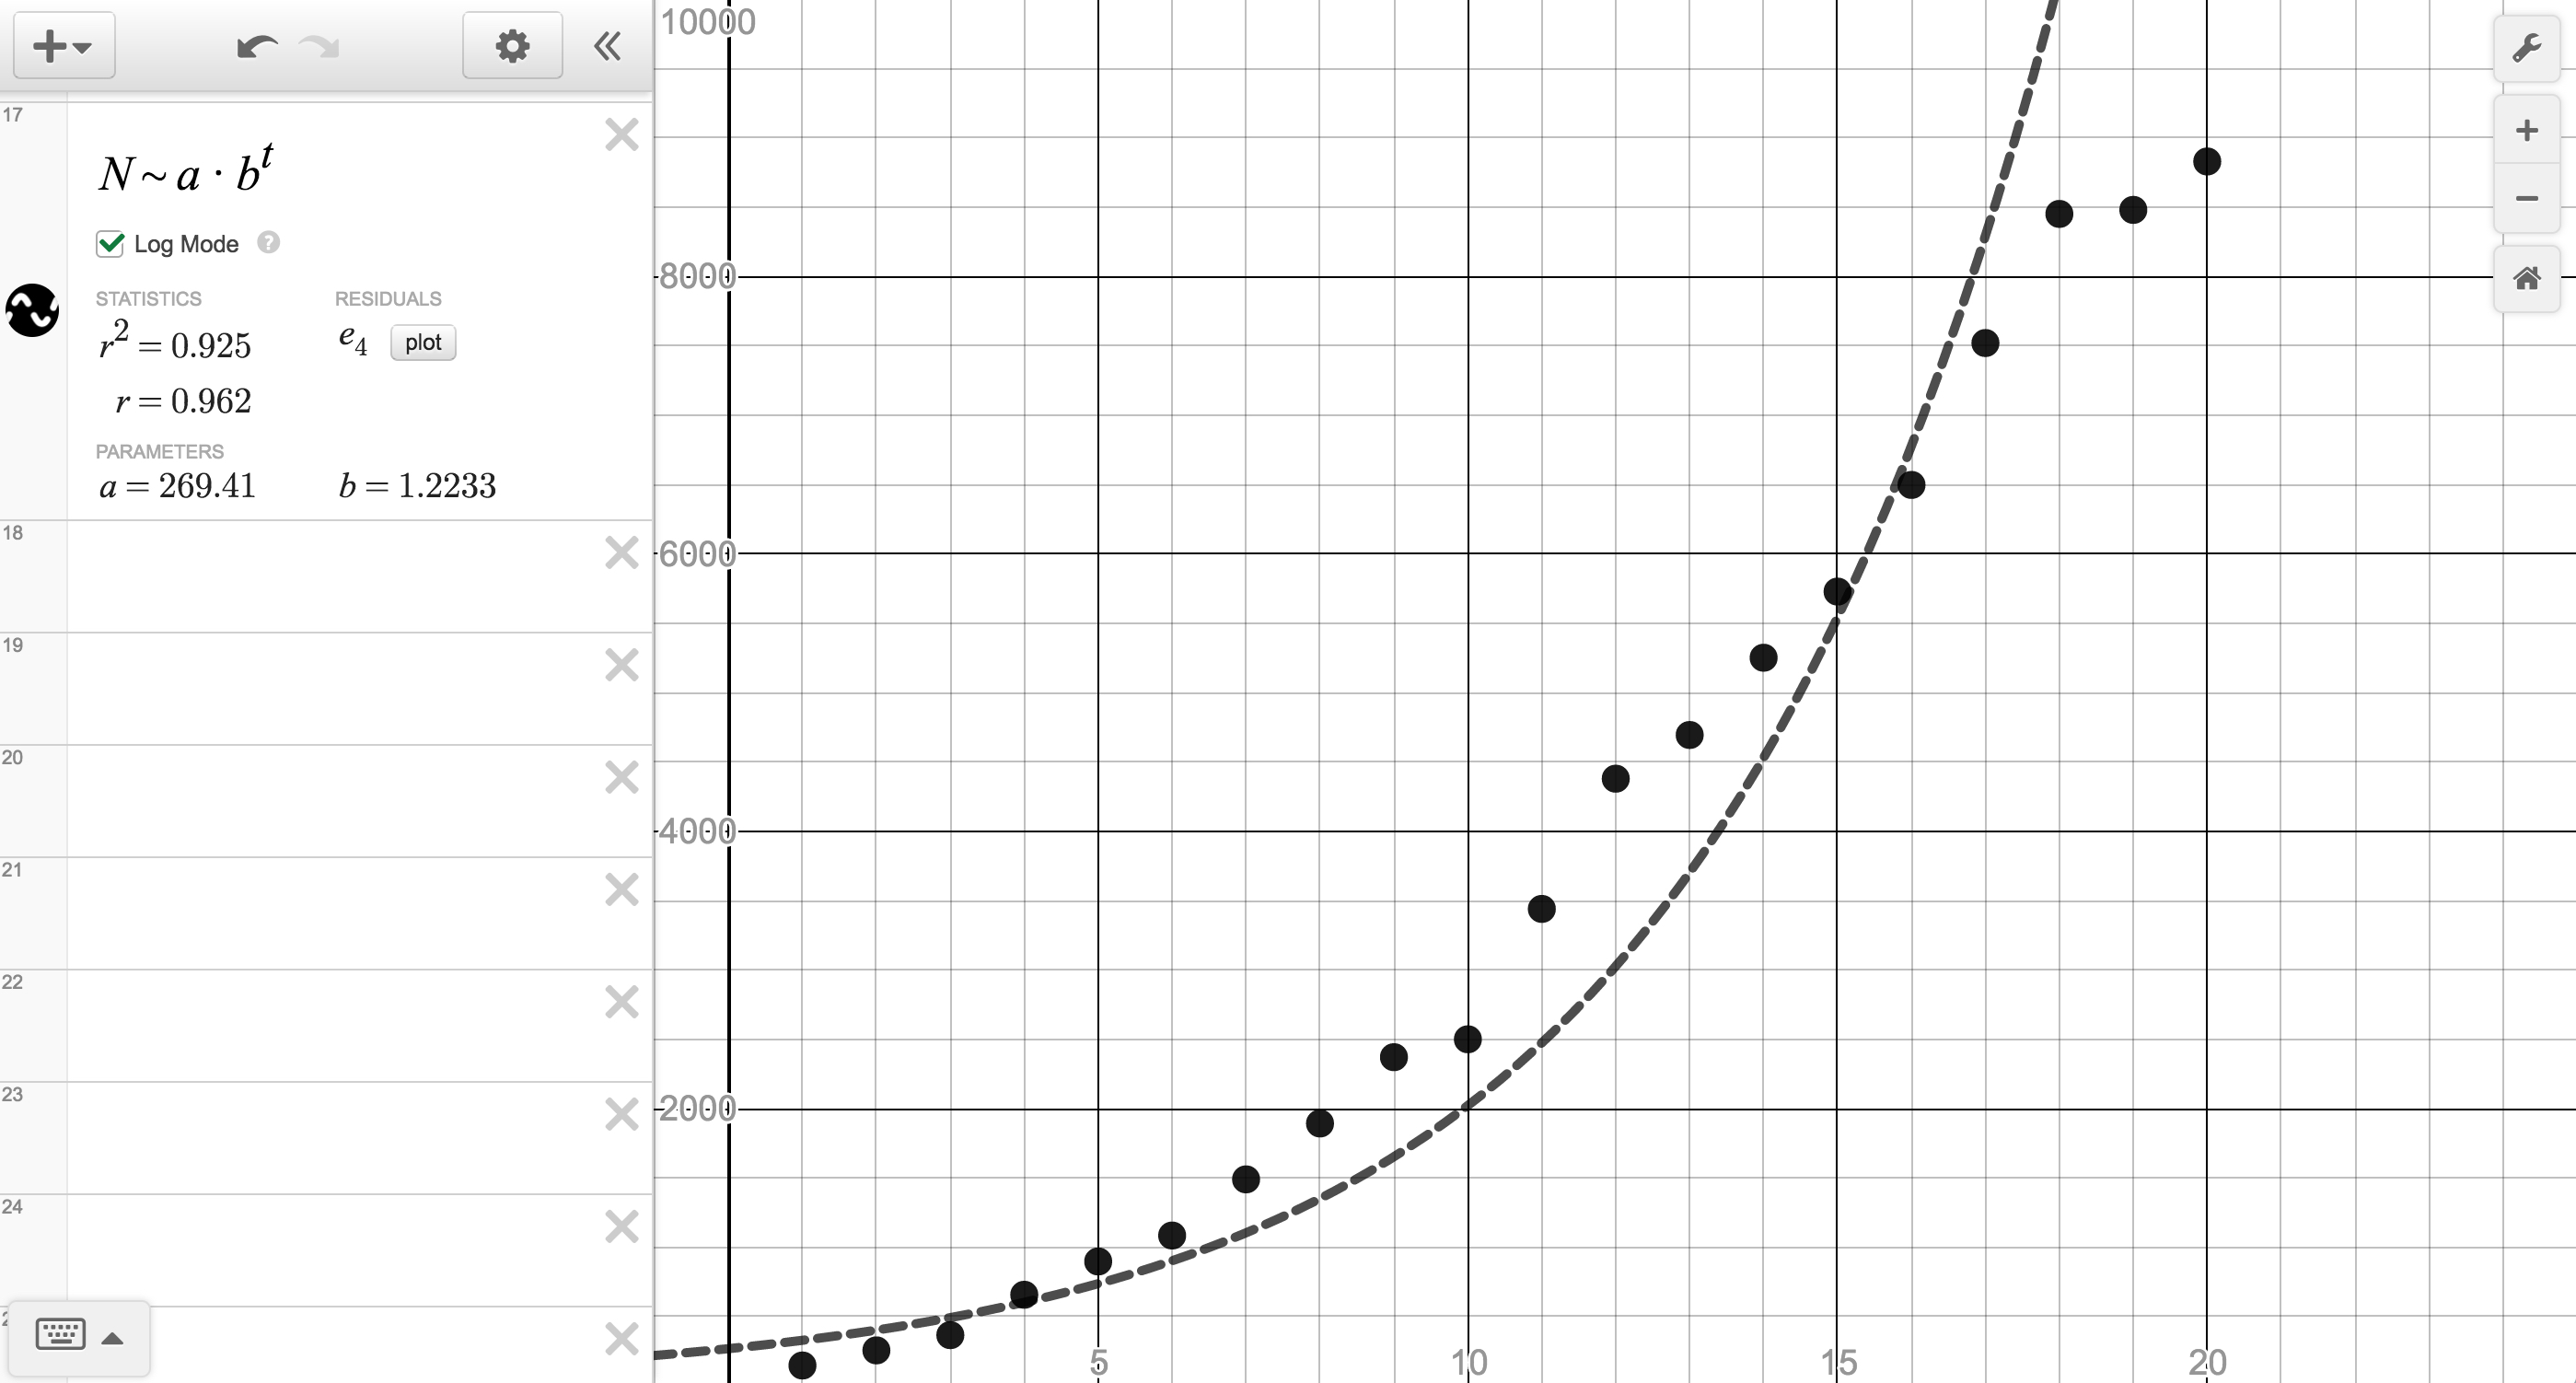
\includegraphics[width=3in]{./ApplicationsofExponentialandLogarithmicFunctionsGraphics/ExpLogAppEx07a.jpg} \\

linear regression: $\ln(N(t)) = t \ln(b) + \ln(a)$ &

exponential regression: $N(t) = a \cdot b^{t}$ \\

\end{tabular}

\end{center}

From the slope of the model, we have   $m = \ln(b) \approx 0.202$  so $b \approx 1.223$.  From the $y$-intercept of the model, we get $B = \ln(a) \approx  5.596$ so $a \approx 269.35$, so that our model is $N(t) = 269.35(1.223)^{t}$. Using the built-in exponential regression (again, with `log mode' checked) returns the model  $N(t) = 269.41 (1.223)^{t}$, the discrepancy between   $269.35$ and $269.41$ stemming ostensibly from round-off error.    

\smallskip

The exponential model didn't fit the data as well as the quadratic or power function model, but it stands to reason that, perhaps, the spread of the flu is not unlike that of the spread of a rumor and that a logistic model can be used to model the data.  Again, for simplicity, we abbreviate the model given in Equation \ref{logisticgrowth} from $N(t) =\frac{L}{1 + Ce^{-kLt}}$ to $N(t) = \frac{L}{1 + Ce^{Kt}}$.

\smallskip

Running the data, a logistic function appears to be an excellent fit, both judging by the graph as well as the coefficient of determination, $R^2 \approx 0.995$.  Moreover, the underlying principles which lead to the formulation of this model seem reasonable enough.




 
 \begin{center}
 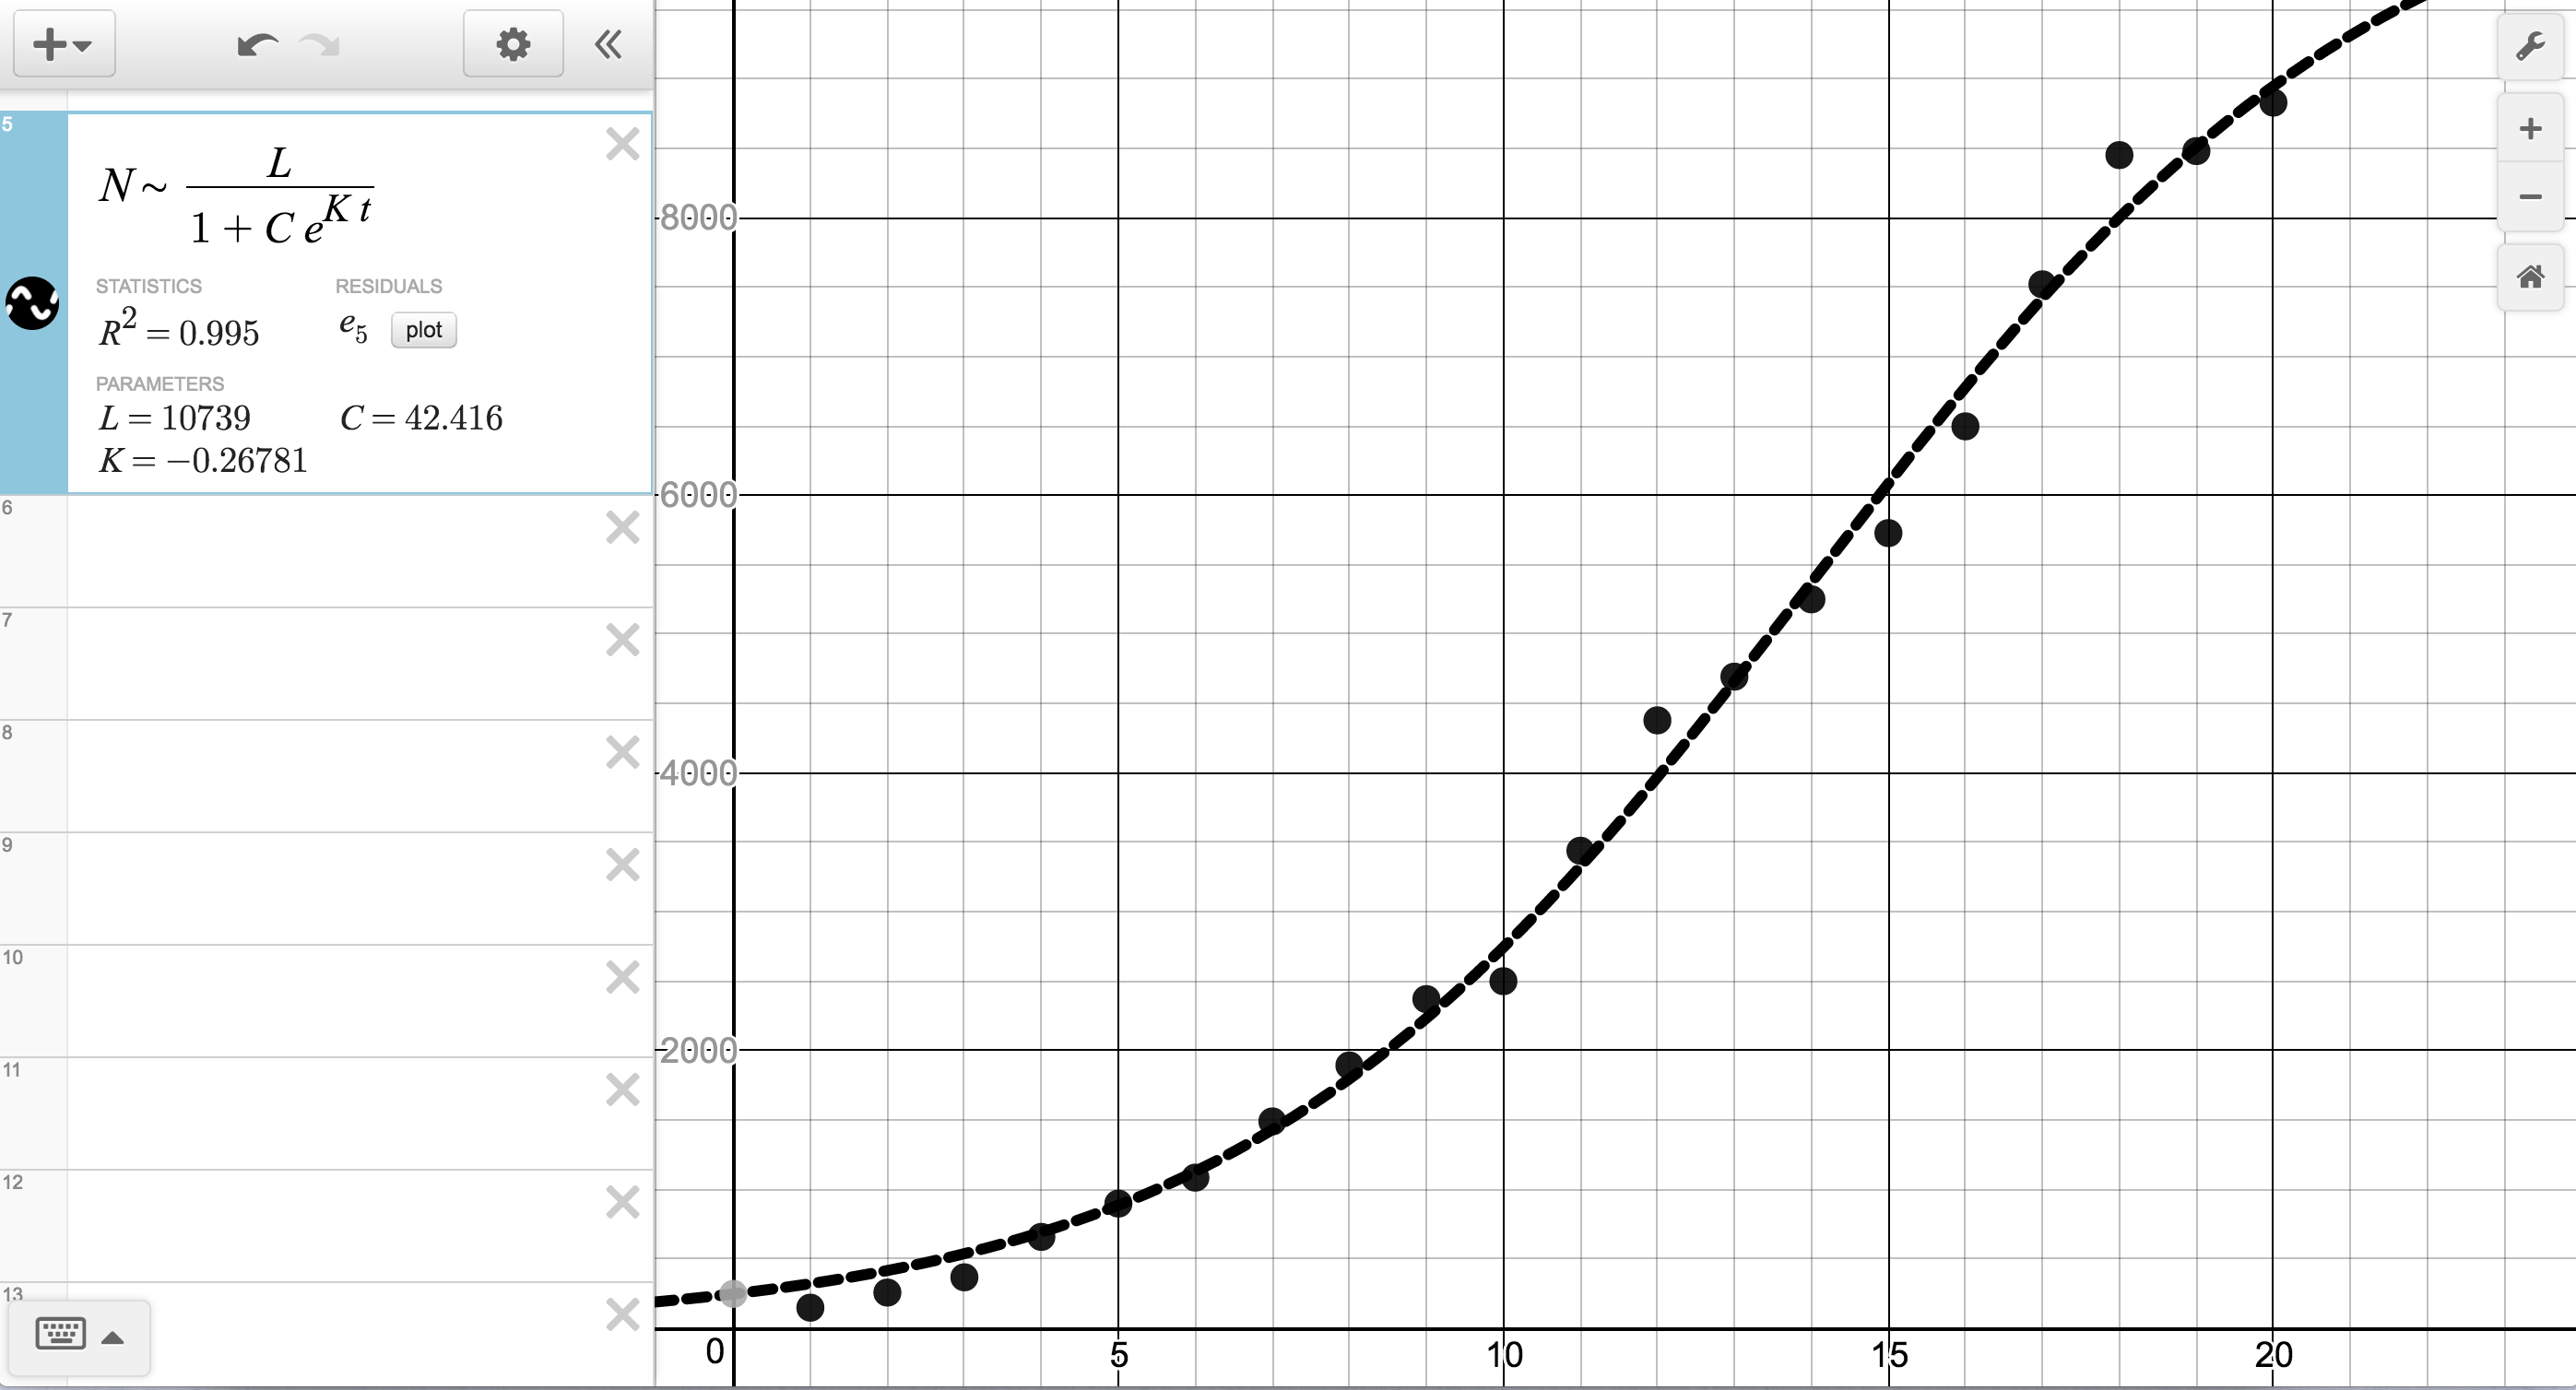
\includegraphics[width=5in]{./ApplicationsofExponentialandLogarithmicFunctionsGraphics/ExpLogAppEx08.jpg} 
 \end{center}



  While the quadratic model also fits extremely well, our logistic model takes into account that only a finite number of people will ever get the flu (according to our model, $L=10,\!739$), whereas the quadratic model predicts no limit to the number of cases. As we have stated several times before in the text, mathematical models, regardless of their sophistication, are just that:  models, and they all have their limitations.\footnote{Speaking of limitations, as of June 3, 2009, there were 19,273 confirmed cases of influenza A (H1N1).  This is well above our prediction of 10,739.  Each time a new report is issued, the data set increases and the model must be recalculated.  We leave this recalculation to the reader.}


\newpage

\subsection{Exercises}

\label{ExercisesforApplicationsofExponentialandLogarithmicFunctions}

For each of the scenarios given in Exercises \ref{basicinterestexfirst} - \ref{basicinterestexlast}, 

\begin{itemize}

\item  Find the amount $A$ in the account as a function of the term of the investment $t$ in years. 

\item  To the nearest cent, determine how much is in the account after $5$, $10$, $30$ and $35$ years.  

\item  To the nearest year, determine how long will it take for the initial investment to double.  

\item  Find and interpret the average rate of change of the amount in the account from the end of
the fourth year to the end of the fifth year, and from the end of the thirty-fourth year to the
end of the thirty-fifth year.  Round your answer to two decimal places.

\end{itemize} 

\begin{enumerate}

\item  $\$500$ is invested in an account which offers $0.75 \%$, compounded monthly. \label{basicinterestexfirst}

\item  $\$500$ is invested in an account which offers $0.75 \%$, compounded continuously.

\item  $\$1000$ is invested in an account which offers $1.25 \%$, compounded monthly.

\item  $\$1000$ is invested in an account which offers $1.25 \%$, compounded continuously.

\item  $\$5000$ is invested in an account which offers $2.125 \%$, compounded monthly.

\item  $\$5000$ is invested in an account which offers $2.125 \%$, compounded continuously. \label{basicinterestexlast}

\setcounter{HW}{\value{enumi}}
\end{enumerate}

\begin{enumerate}
\setcounter{enumi}{\value{HW}}

\item  Look back at your answers to Exercises \ref{basicinterestexfirst} - \ref{basicinterestexlast}. What can be said about the difference between monthly compounding and continuously compounding the interest in those situations?  With the help of your classmates, discuss scenarios where the difference between monthly  and continuously compounded interest would be more dramatic.  Try varying the interest rate, the term of the investment and the principal.  Use computations to support your answer.

\item  How much money needs to be invested now to obtain $\$2000$ in 3 years if the interest rate in a savings account is $0.25 \%$, compounded continuously?  Round your answer to the nearest cent.

\item  How much money needs to be invested now to obtain $\$5000$ in  10 years if the interest rate in a CD is $2.25 \%$, compounded monthly?  Round your answer to the nearest cent.


\item On May, 31, 2009, the Annual Percentage Rate listed at Jeff's bank for regular savings accounts was $0.25\%$ compounded monthly.  Use Equation \ref{compoundinterest} to answer the following.

\begin{enumerate}

\item If $P = 2000$ what is $A(8)$?
\item Solve the equation $A(t) = 4000$ for $t$.
\item What principal $P$ should be invested so that the account balance is \$2000 is three years?

\end{enumerate}

\pagebreak

\item Jeff's bank also offers a 36-month Certificate of Deposit (CD) with an APR of $2.25\%$.

\begin{enumerate}

\item If $P = 2000$ what is $A(8)$?
\item Solve the equation $A(t) = 4000$ for $t$.
\item What principal $P$ should be invested so that the account balance is \$2000 in three years?
\item The Annual Percentage Yield is the \underline{simple} interest rate that returns the same amount of interest after one year as the compound interest does.  With the help of your classmates, compute the APY for this investment.

\end{enumerate}


\item  A finance company offers a promotion on $\$5000$ loans.  The borrower does not have to make any payments for the first three years, however interest will continue to be charged to the loan at $29.9 \%$ compounded continuously.  What amount will be due at the end of the three year period, assuming no payments are made?  If the promotion is extended an additional three years, and no payments are made, what amount would be due?

\item Use Equation \ref{compoundinterest} to show that the time it takes for an investment to double in value does \underline{not} depend on the principal $P$, but rather, depends only on the APR and the number of compoundings per year.  Let $n = 12$ and with the help of your classmates compute the doubling time for a variety of rates $r$.  Then look up the Rule of 72 and compare your answers to what that rule says.  If you're really interested\footnote{Awesome pun!} in Financial Mathematics, you could also compare and contrast the Rule of 72 with the Rule of 70 and the Rule of 69.

\setcounter{HW}{\value{enumi}}
\end{enumerate}

In Exercises \ref{radioactivefirst} - \ref{radioactivelast},  we list some radioactive isotopes and their associated half-lives.  Assume that each decays according to the formula $A(t) = A_{\text{\tiny $0$}}e^{kt}$ where $A_{\text{\tiny $0$}}$ is the initial amount of the material and $k$ is the decay constant. For each isotope:

\begin{itemize}

\item  Find the decay constant $k$.  Round your answer to four decimal places.

\item  Find a function which gives the amount of isotope $A$ which remains after time $t$.  (Keep the units of $A$ and $t$ the same as the given data.)

\item  Determine how long it takes for $90 \%$ of the material to decay.  Round your answer to two decimal places.  (HINT:  If $90 \%$ of the material decays, how much is left?)

\end{itemize}

\begin{enumerate}
\setcounter{enumi}{\value{HW}}

\item  Cobalt 60, used in food irradiation, initial amount 50 grams, half-life of $5.27$ years.  \label{radioactivefirst}

\item  Phosphorus 32, used in agriculture, initial amount 2 milligrams, half-life $14$ days.

\item  Chromium 51, used to track red blood cells, initial amount 75 milligrams, half-life  $27.7$ days.

\item  Americium 241, used in smoke detectors, initial amount 0.29 micrograms, half-life $432.7$ years.

\item  Uranium 235, used for nuclear power, initial amount $1$ kg grams, half-life  $704$ million years. \label{radioactivelast}

\setcounter{HW}{\value{enumi}}
\end{enumerate}

\begin{enumerate}
\setcounter{enumi}{\value{HW}}

\item With the help of your classmates, show that the time it takes for $90 \%$ of each isotope listed in Exercises \ref{radioactivefirst} - \ref{radioactivelast} to decay does not depend on the initial amount of the substance, but rather, on only the decay constant $k$. Find a formula, in terms of $k$ only, to determine how long it takes for $90 \%$ of a radioactive isotope to decay. 


\item In Example \ref{cardepreciationex} in Section \ref{ExponentialFunctions}, the exponential function $V(x) = 25 \left(\frac{4}{5}\right)^{x}$ was used to model the value of a car over time.  Use a change of base formula to rewrite the model in the form $V(t) = 25e^{kt}$.

\item  The Gross Domestic Product (GDP) of the US (in billions of dollars) $t$ years after the year 2000 can be modeled by: \[ G(t) = 9743.77 e^{0.0514t}\]

\begin{enumerate}

\item  Find and interpret $G(0)$.

\item  According to the model, what should have been the GDP in 2007?  In 2010?  (According to the   \href{http://1.usa.gov/iimT40}{\underline{US Department of Commerce}}, the 2007 GDP was $\$14,369.1$ billion and the 2010 GDP was $\$14,657.8$ billion.)

\end{enumerate}

\item  The diameter $D$ of a tumor, in millimeters, $t$ days after it is detected is given by:  \[D(t) = 15e^{0.0277t} \]

\begin{enumerate}

\item  What was the diameter of the tumor when it was originally detected?

\item  How long until the diameter of the tumor doubles?

\end{enumerate}

\item  Under optimal conditions, the growth of a certain strain of \textit{E. Coli} is modeled by the Law of Uninhibited Growth $N(t) = N_{\text{\tiny $0$}} e^{kt}$ where $N_{\text{\tiny $0$}}$ is the initial number of bacteria and $t$ is the elapsed time, measured in minutes. From numerous experiments, it has been determined that the doubling time of this organism is 20 minutes. Suppose 1000 bacteria are present initially.

\begin{enumerate}

\item  Find the growth constant $k$. Round your answer to four decimal places.

\item  Find a function which gives the number of bacteria $N(t)$ after $t$ minutes.

\item  How long until there are 9000 bacteria?  Round your answer to the nearest minute.

\end{enumerate}

\item  Yeast is often used in biological experiments.  A research technician estimates that a sample of yeast suspension contains 2.5 million organisms per cubic centimeter (cc).  Two hours later, she estimates the population density to be 6 million organisms per cc.  Let $t$ be the time elapsed since the first observation, measured in hours.  Assume that the yeast growth follows the Law of Uninhibited Growth $N(t) = N_{\text{\tiny $0$}} e^{kt}$.

\begin{enumerate}

\item  Find the growth constant $k$. Round your answer to four decimal places.

\item  Find a function which gives the number of yeast (in millions) per cc $N(t)$ after $t$ hours.

\item  What is the doubling time for this strain of yeast?

\end{enumerate}


\item  The Law of Uninhibited Growth also applies to situations where an animal is re-introduced into a suitable environment.  Such a case is the reintroduction of wolves to Yellowstone National Park.   According to the \href{http://www.nps.gov/yell/naturescience/wolves.htm}{\underline{National Park Service}}, the wolf population in Yellowstone National Park was 52 in 1996 and 118 in 1999.  Using these data, find a function of the form $N(t) = N_{\text{\tiny $0$}} e^{kt}$  which models the number of wolves $t$ years after 1996.  (Use $t = 0$ to represent the year 1996.  Also, round your value of $k$ to four decimal places.)  According to the model, how many wolves were in Yellowstone in 2002?  (The recorded number is 272.)

\item  \label{PainesvillePopulationTwoPoint} During the early years of a community, it is not uncommon for the population to grow according to the Law of Uninhibited Growth.  According to the Painesville Wikipedia entry, in 1860, the Village of Painesville had a population of 2649.  In 1920, the population was 7272.  Use these two data points to fit a model of the form $N(t) = N_{\text{\tiny $0$}} e^{kt}$ were $N(t)$ is the number of Painesville Residents $t$ years after 1860.  (Use $t = 0$ to represent the year 1860.  Also, round the value of $k$ to four decimal places.)  According to this model, what was the population of Painesville in 2010?  (The 2010 census gave the population as 19,563) What could be some causes for such a vast discrepancy?  For more on this, see Exercise \ref{PainesvillePopulationManyPoints}.

\item  The population of Sasquatch in Bigfoot county is modeled by \[P(t) = \dfrac{120}{1 + 3.167e^{-0.05t}}\] where $P(t)$ is the population of Sasquatch $t$ years after $2010$.

\begin{enumerate}

\item  Find and interpret $P(0)$.

\item  Find the population of Sasquatch in Bigfoot county in 2013 rounded to the nearest Sasquatch.

\item  To the nearest year, when will the population of Sasquatch in Bigfoot county reach 60?  

\item   Find and interpret the end behavior of the graph of $y = P(t)$ analytically. Check your answer using a graphing utility. 

\end{enumerate}

\setcounter{HW}{\value{enumi}}
\end{enumerate}


\begin{enumerate}
\setcounter{enumi}{\value{HW}}

\item  Let $f(x) = \dfrac{10}{1+e^{-x+1}}$.   

\begin{enumerate}

\item From Calculus, we know the inflection point of the graph of $y=f(x)$ is $(1,5)$.  This means the function is increasing the fastest at $x=1$, or, equivalently, the slope at $(1,5)$ is the largest anywhere on the graph.  Graph $y=f(x)$ using a graphing utility and convince yourself of the reasonableness of this claim.

\item Find average rate of change of $f$ over each of the intervals below.  What do you guess the slope of the curve is at $(1,5)$?  Zoom in on the graph near $(1,5)$ to check your guess.

\begin{multicols}{6}

\begin{itemize}

\item $[0.75, 1]$

\item $[0.9, 1]$

\item $[0.99,1]$

\item $[1, 1.01]$

\item $[1, 1.1]$

\item $[1, 1.25]$

\end{itemize}

\end{multicols}

\end{enumerate}

\newpage


\item The half-life of the radioactive isotope Carbon-14 is about 5730 years.  

\begin{enumerate}

\item Use Equation \ref{radioactivedecay} to express the amount of Carbon-14 left from an initial $N$ milligrams as a function of time $t$ in years.

\item What percentage of the original amount of Carbon-14 is left after 20,000 years?

\item If an old wooden tool is found in a cave and the amount of Carbon-14 present in it is estimated to be only 42\% of the original amount, approximately how old is the tool?

\item Radiocarbon dating is not as easy as these exercises might lead you to believe.  With the help of your classmates, research radiocarbon dating and discuss why our model is somewhat over-simplified.  

\end{enumerate}

\item Carbon-14 cannot be used to date inorganic material such as rocks, but there are many other methods of radiometric dating which estimate the age of rocks.  One of them, Rubidium-Strontium dating, uses Rubidium-87 which decays to Strontium-87 with a half-life of 50 billion years.  Use Equation \ref{radioactivedecay} to express the amount of Rubidium-87 left from an initial 2.3 micrograms as a function of time $t$ in \emph{billions} of years.  Research this and other radiometric techniques and discuss the margins of error for various methods with your classmates.

\item  Find and interpret the relative rate of change of  $A(t)$ in Equation \ref{compoundinterest} over the interval $\left[t, t+\frac{1}{n} \right]$.

\item Use Equation \ref{radioactivedecay} to show that $k = -\dfrac{\ln(2)}{h}$ where $h$ is the half-life of the radioactive isotope.

\item A pork roast\footnote{This roast was enjoyed by Jeff and his family on June 10, 2009.  This is real data, folks!} was taken out of a hardwood smoker when its internal temperature had reached $180^{\circ}$F and it was allowed to rest in a $75^{\circ}$F house for 20 minutes after which its internal temperature had dropped to $170^{\circ}$F. 

Assuming that the temperature of the roast follows Newton's Law of Cooling (Equation \ref{newtonslawofcooling}),

\begin{enumerate}

\item Express the temperature $T$ (in $^{\circ}$F) as a function of time $t$ (in minutes).

\item Find the time at which the roast would have dropped to $140^{\circ}$F had it not been eaten. 

\end{enumerate}

\item  \label{pursuitlog} In reference to Exercise \ref{pursuitfurther} in Section \ref{PowerFunctions}, if Fritzy the Fox's speed is the same as Chewbacca the Bunny's speed, Fritzy's pursuit curve is given by

\[y(x) = \frac{1}{4} x^2-\frac{1}{4} \ln(x)-\frac{1}{4}\]

Graph this path for $x > 0$ using a graphing utility.  Describe the behavior of $y$ as $x \rightarrow 0^{+}$ and interpret this physically.

\item \label{explogsappcircuitone} The current $i$ measured in amps in a certain electronic circuit with a constant impressed voltage of 120 volts is given by $i(t) = 2 - 2e^{-10t}$ where $t \geq 0$ is the number of seconds after the circuit is switched on.  Determine the value of $i$ as $t \rightarrow \infty$.  (This is called the \textbf{steady state} current.)


\item If the voltage in the circuit in Exercise \ref{explogsappcircuitone} above is switched off after 30 seconds, the current is given by the piecewise-defined function 

\[i(t) = \left\{ \begin{array}{rcl} 2 - 2e^{-10t} & \mbox{if} & 0 \leq t < 30 \\ [6pt]
\left(2 - 2e^{-300}\right) e^{-10t+300} & \mbox{if} & t \geq 30 \end{array} \right.\]  

With the help of a graphing utility, graph $y = i(t)$ and discuss with your classmates the physical significance of the two parts of the graph $0 \leq t < 30$ and $t \geq 30$.


\item \label{catenary} In Exercise \ref{parabolicbridgecable} in Section \ref{QuadraticFunctions}, we stated that the cable of a suspension bridge formed a parabola but that a free hanging cable did not.  A free hanging cable forms a \underline{catenary} and its basic shape is given by $y = \frac{1}{2}\left(e^{x} + e^{-x}\right)$.  Use a graphing utility to graph this function.  What are its domain and range?  What is its end behavior?  Is it invertible?  How do you think it is related to the function given in Exercise \ref{hyperbolicsine} in Section \ref{ExponentialEquationsandInequalities} and the one given in the answer to Exercise \ref{inversehyptangent} in Section \ref{LogarithmicEquationsandInequalities}?  

When flipped upside down, the catenary makes an arch.  The Gateway Arch in St. Louis, Missouri has the shape \[y = 757.7 - \frac{127.7}{2}\left(e^{\frac{x}{127.7}} + e^{-\frac{x}{127.7}}\right)\] where $x$ and $y$ are measured in feet and $-315 \leq x \leq 315$.  Find the highest point on the arch.

\item \label{APLcatsrevisited} In Exercise \ref{APLcats} in Section \ref{QuadraticFunctions}, we examined the data set given below which showed how two cats and their surviving offspring can produce over 80 million cats in just ten years. Plot $x$ versus $\ln(x)$ as was done on page \pageref{swineflulinearized} using a graphing utility.  

Find a linear model for this new data and comment on its goodness of fit and  find an exponential model for the original data and comment on its goodness of fit.

\medskip

\small

\noindent \begin{tabular}{|l|r|r|r|r|r|r|r|r|r|r|} \hline
Year $x$ & 1 & 2 & 3 & 4 & 5 & 6 & 7 & 8 & 9 & 10 \\ 
\hline 
Number of  & & & & & & & & & & \\
Cats $N(x)$ & 12 & 66 & 382 & 2201 & 12680 & 73041 & 420715 & 2423316 & 13968290 & 80399780 \\ \hline
\end{tabular}

\normalsize

\item \label{LorenzExFollowUp} In Example \ref{LorenzEx} in Section \ref{PowerFunctions}, we fit a power function of the form $L(x) = a x^{p}$ to a set of data, $(x, L(x))$.  In this exercise, we use logs to linearize this data using the same methods presented on page \pageref{swineflulinearized}, but with a slight difference in interpretation.

\begin{enumerate}

\item  Starting with $L(x) = a x^{p}$, take natural logs of both sides of the equation and use log properties to rewrite the resulting equation as:  $\ln(L(x)) = p \ln(x) + \ln(a)$.  

\item  Use a graphing utility to find a least squares regression line using the data $(\ln(x), \ln(L(x)))$.   

NOTE:  In this situation, we are plotting $\ln(x)$ versus $\ln(L(x))$ instead of $x$ versus $\ln(L(x))$.  

\item  \label{newlorenzepart} Find the slope $p$ of the regression line and the intercept $\ln(a)$.  Use these to construct a model of the form $L(x) = a x^{p}$.   Find and interpret $L(90)$.

\item   Graph both the model obtained in Example \ref{LorenzEx} and the model obtained in part \ref{newlorenzepart} along with the original data.  What do you notice?

\end{enumerate}

\item  \label{PainesvillePopulationManyPoints} This exercise is a follow-up to Exercise \ref{PainesvillePopulationTwoPoint} which more thoroughly explores the population growth of Painesville, Ohio.  According to \href{http://en.wikipedia.org/wiki/Painesville}{\underline{Wikipedia}}, the population of Painesville, Ohio is given by


\noindent \begin{tabular}{|l|r|r|r|r|r|r|r|r|r|r|} \hline
Year $t$ & 1860 & 1870 & 1880 & 1890 & 1900 & 1910 & 1920 & 1930 & 1940 & 1950 \\ \hline 
Population& 2649 & 3728 & 3841 & 4755 & 5024 & 5501 & 7272 & 10944 & 12235 & 14432 \\ \hline
\end{tabular}

\noindent \begin{tabular}{|l|r|r|r|r|r|} \hline
Year $t$ & 1960 & 1970 & 1980 & 1990 & 2000 \\ \hline 
Population& 16116 & 16536 & 16351 & 15699 & 17503 \\ \hline
\end{tabular}

\begin{enumerate}

\item  Use a graphing utility to perform an exponential regression on the data from 1860 through 1920 only, letting $t = 0$ represent the year 1860 as before.  How does this model compare with the model you found in Exercise \ref{PainesvillePopulationTwoPoint}?   Use the graphing utility's exponential model to predict the population in 2010.   (The 2010 census gave the population as 19,563)

\item  The logistic model fit to \emph{all} of the given data points for the population of Painesville $t$ years after 1860 (again, using $t = 0$ as 1860) is \[ P(t) = \dfrac{18691}{1+9.8505e^{-0.03617t}} \] According to this model, what should the population of Painesville have been in 2010?  (The 2010 census gave the population as 19,563.) What is the population limit of Painesville?

\end{enumerate}

\item  According to \href{http://www.ohiobiz.com/census/Lake.pdf}{\underline{OhioBiz}}, the census data for Lake County, Ohio is as follows:

\small
\noindent \begin{tabular}{|l|r|r|r|r|r|r|r|r|r|r|} \hline
Year $t$ & 1860 & 1870 & 1880 & 1890 & 1900 & 1910 & 1920 & 1930 & 1940 & 1950 \\ \hline 
Population& 15576 & 15935 & 16326 & 18235 & 21680 & 22927 & 28667 & 41674 & 50020 & 75979 \\ \hline
\end{tabular}

\noindent \begin{tabular}{|l|r|r|r|r|r|} \hline
Year $t$ & 1960 & 1970 & 1980 & 1990 & 2000 \\ \hline 
Population& 148700 & 197200 & 212801 & 215499 & 227511 \\ \hline
\end{tabular}

\normalsize

\begin{enumerate}

\item  Use a graphing utility to fit a logistic model to these data with $x = 0$ representing the year 1860. 

\item  Graph the data and your model using a graphing utility to judge the reasonableness of the fit.

\item  Use this model to estimate the population of Lake County in 2010.  (The 2010 census gave the population to be 230,041.)

\item  According to your model, what is the population limit of Lake County, Ohio?

\end{enumerate}


\item According to \href{http://www.facebook.com/press/info.php?timeline}{\underline{facebook}}, the number of active users of facebook has grown significantly since its initial launch from a Harvard dorm room in February 2004. The chart below has the approximate number $U(x)$ of active users, in \underline{millions}, $x$ months after February 2004.  For example, the first entry $(10, 1)$ means that there were $1$ million active users in December 2004 and the last entry $(77, 500)$ means that there were $500$ million active users in July 2010.

\medskip
\small
\noindent \begin{tabular}{|l|r|r|r|r|r|r|r|r|r|r|r|r|r|r|} \hline
Month $x$ & 10 & 22 & 34 & 38 & 44 & 54 & 59 & 60 & 62 & 65 & 67 & 70 & 72 & 77 \\ \hline 
Active Users in & & & & & & & & & & & & & & \\
Millions $U(x)$ & 1 & 5.5 & 12 & 20 & 50 & 100 & 150 & 175 & 200 & 250 & 300 & 350 & 400 & 500\\ \hline
\end{tabular}
\normalsize
\medskip

  With the help of your classmates, find a model for this data.


\item Each Monday during the registration period before the Fall Semester at LCCC, the Enrollment Planning Council gets a report prepared by the data analysts in Institutional Effectiveness and Planning.\footnote{Thanks to Dr. Wendy Marley and her staff for this data and Dr. Marcia Ballinger for the permission to use it  in this problem.}  While the ongoing enrollment data is analyzed in many different ways, we shall focus only on the overall headcount.  Below is a chart of the enrollment data for Fall Semester 2008.  It starts 21 weeks before ``Opening Day'' and ends on ``Day 15'' of the semester, but we have relabeled the top row to be $x = 1$ through $x = 24$ so that the math is easier.  (Thus, $x = 22$ is Opening Day.)


\noindent \begin{tabular}{|l|r|r|r|r|r|r|r|r|} \hline
Week $x$ & 1 & 2 & 3 & 4 & 5 & 6 & 7 & 8 \\ \hline 
Total  & & & & & & & & \\
Headcount & 1194 & 1564 & 2001 & 2475 & 2802 & 3141 & 3527 & 3790 \\ \hline
\end{tabular}

\medskip

\noindent \begin{tabular}{|l|r|r|r|r|r|r|r|r|} \hline
Week $x$ & 9 & 10 & 11 & 12 & 13 & 14 & 15 & 16 \\ \hline 
Total  & & & & & & & & \\
Headcount & 4065 & 4371 & 4611 & 4945 & 5300 & 5657 & 6056 & 6478 \\ \hline
\end{tabular}

\medskip

\noindent \begin{tabular}{|l|r|r|r|r|r|r|r|r|} \hline
Week $x$ & 17 & 18 & 19 & 20 & 21 & 22 & 23 & 24\\ \hline 
Total  & & & & & & & & \\
Headcount & 7161 & 7772 & 8505 & 9256 & 10201 & 10743 & 11102 & 11181 \\ \hline
\end{tabular}

\medskip

With the help of your classmates, find a model for this data.  Unlike most of the phenomena we have studied in this section, there is no single differential equation which governs the enrollment growth.  Thus there is no scientific reason to rely on a logistic function even though the data plot may lead us to that model.  What are some factors which influence enrollment at a community college and how can you take those into account mathematically?  

\item When we wrote this exercise, the Enrollment Planning Report for Fall Semester 2009 had only 10 data points for the first 10 weeks of the registration period.  Those numbers are given below.  

\noindent \begin{tabular}{|l|r|r|r|r|r|r|r|r|r|r|} \hline
Week $x$ & 1 & 2 & 3 & 4 & 5 & 6 & 7 & 8 & 9 & 10 \\ \hline 
Total  & & & & & & & & & & \\
Headcount & 1380 & 2000 & 2639 & 3153 & 3499 & 3831 & 4283 & 4742 & 5123 & 5398 \\ \hline
\end{tabular}

With the help of your classmates, find a model for this data and make a prediction for the Opening Day enrollment as well as the Day 15 enrollment.  (WARNING: The registration period for 2009 was one week shorter than it was in 2008 so Opening Day would be $x = 21$ and Day 15 is $x = 23$.)


\end{enumerate}

\newpage

\subsection{Answers}

\begin{enumerate}

\item \begin{itemize}  \item $A(t) = 500\left(1 + \frac{0.0075}{12}\right)^{12t}$ 

\item $A(5) \approx \$ 519.10$, $A(10) \approx \$ 538.93$, $A(30) \approx \$ 626.12$, $A(35) \approx \$ 650.03$ 

\item It will take approximately $92$ years for the investment to double.

\item  The average rate of change from the end of the fourth year to the end of the fifth year is approximately $3.88$.  This means that the investment is growing at an average rate of $\$3.88$ per year at this point.  The average rate of change from the end of the thirty-fourth year to the end of the thirty-fifth year is approximately $4.85$.  This means that the investment is growing at an average rate of $\$4.85$ per year at this point. 

\end{itemize}

\item \begin{itemize}  \item $A(t) = 500e^{0.0075t}$ 

\item $A(5) \approx \$ 519.11$, $A(10) \approx \$ 538.94$, $A(30) \approx \$ 626.16$, $A(35) \approx \$ 650.09$ 

\item It will take approximately $92$ years for the investment to double.

\item  The average rate of change from the end of the fourth year to the end of the fifth year is approximately $3.88$.  This means that the investment is growing at an average rate of $\$3.88$ per year at this point.  The average rate of change from the end of the thirty-fourth year to the end of the thirty-fifth year is approximately $4.86$.  This means that the investment is growing at an average rate of $\$4.86$ per year at this point. 

\end{itemize}

\item \begin{itemize}  \item $A(t) = 1000\left(1 + \frac{0.0125}{12}\right)^{12t}$ 

\item $A(5) \approx \$ 1064.46$, $A(10) \approx \$ 1133.07$, $A(30) \approx \$ 1454.71$, $A(35) \approx \$ 1548.48$ 

\item  It will take approximately $55$ years for the investment to double.

\item  The average rate of change from the end of the fourth year to the end of the fifth year is approximately $13.22$.  This means that the investment is growing at an average rate of $\$13.22$ per year at this point.  The average rate of change from the end of the thirty-fourth year to the end of the thirty-fifth year is approximately $19.23$.  This means that the investment is growing at an average rate of $\$19.23$ per year at this point. 

\end{itemize}



\item \begin{itemize}  \item $A(t) = 1000e^{0.0125t}$ 

\item $A(5) \approx \$ 1064.49$, $A(10) \approx \$ 1133.15$, $A(30) \approx \$ 1454.99$, $A(35) \approx \$ 1548.83$ 

\item It will take approximately $55$ years for the investment to double.

\item  The average rate of change from the end of the fourth year to the end of the fifth year is approximately $13.22$.  This means that the investment is growing at an average rate of $\$13.22$ per year at this point.  The average rate of change from the end of the thirty-fourth year to the end of the thirty-fifth year is approximately $19.24$.  This means that the investment is growing at an average rate of $\$19.24$ per year at this point. 

\end{itemize}

\pagebreak

\item \begin{itemize}  \item $A(t) = 5000\left(1 + \frac{0.02125}{12}\right)^{12t}$ 

\item $A(5) \approx \$ 5559.98$, $A(10) \approx \$ 6182.67$, $A(30) \approx \$ 9453.40$, $A(35) \approx \$ 10512.13$ 

\item  It will take approximately $33$ years for the investment to double.

\item  The average rate of change from the end of the fourth year to the end of the fifth year is approximately $116.80$.  This means that the investment is growing at an average rate of $\$116.80$ per year at this point.  The average rate of change from the end of the thirty-fourth year to the end of the thirty-fifth year is approximately $220.83$.  This means that the investment is growing at an average rate of $\$220.83$ per year at this point. 

\end{itemize}



\item \begin{itemize}  \item $A(t) = 5000e^{0.02125t}$ 

\item $A(5) \approx \$ 5560.50$, $A(10) \approx \$ 6183.83$, $A(30) \approx \$ 9458.73$, $A(35) \approx \$ 10519.05$ 

\item  It will take approximately $33$ years for the investment to double.

\item  The average rate of change from the end of the fourth year to the end of the fifth year is approximately $116.91$.  This means that the investment is growing at an average rate of $\$116.91$ per year at this point.  The average rate of change from the end of the thirty-fourth year to the end of the thirty-fifth year is approximately $221.17$.  This means that the investment is growing at an average rate of $\$221.17$ per year at this point. 

\end{itemize}

\setcounter{HW}{\value{enumi}}
\end{enumerate}

\begin{enumerate}
\setcounter{enumi}{\value{HW}}

\addtocounter{enumi}{1}

\item  $P = \frac{2000}{e^{0.0025 \cdot 3}} \approx \$ 1985.06$

\item  $P = \frac{5000}{\left(1 + \frac{0.0225}{12}\right)^{12 \cdot 10}} \approx \$ 3993.42$

\item \begin{enumerate}

\item $A(8) = 2000\left(1 + \frac{0.0025}{12}\right)^{12 \cdot 8} \approx \$2040.40$
\item $t = \dfrac{\ln(2)}{12 \ln\left(1 + \frac{0.0025}{12}\right)} \approx 277.29$ years
\item $P = \dfrac{2000}{\left(1 + \frac{0.0025}{12}\right)^{36}} \approx \$1985.06$

\end{enumerate}

\item \begin{enumerate}

\item $A(8) = 2000\left(1 + \frac{0.0225}{12}\right)^{12 \cdot 8} \approx \$2394.03$
\item $t = \dfrac{\ln(2)}{12 \ln\left(1 + \frac{0.0225}{12}\right)} \approx 30.83$ years
\item $P = \dfrac{2000}{\left(1 + \frac{0.0225}{12}\right)^{36}} \approx \$1869.57$
\item $\left(1 + \frac{0.0225}{12}\right)^{12} \approx 1.0227$ so the APY is 2.27\%

\end{enumerate}

\item  $A(3) = 5000e^{0.299 \cdot 3} \approx \$12,226.18$,  $A(6) = 5000e^{0.299 \cdot 6} \approx \$30,067.29$

\setcounter{HW}{\value{enumi}}
\end{enumerate}


\begin{multicols}{2}
\begin{enumerate}
\setcounter{enumi}{\value{HW}}
\addtocounter{enumi}{1}

\item  \begin{itemize}  \item $k = \frac{\ln(1/2)}{5.27} \approx -0.1315$

\item $A(t) = 50e^{-0.1315t}$

\item  $t = \frac{\ln(0.1)}{-0.1315} \approx 17.51$ years.

\end{itemize}



\item  \begin{itemize}  \item $k = \frac{\ln(1/2)}{14} \approx -0.0495$

\item $A(t) = 2e^{-0.0495t}$

\item  $t = \frac{\ln(0.1)}{-0.0495} \approx 46.52$ days.

\end{itemize}

\setcounter{HW}{\value{enumi}}
\end{enumerate}
\end{multicols}

\begin{multicols}{2}
\begin{enumerate}
\setcounter{enumi}{\value{HW}}


\item  \begin{itemize}  \item $k = \frac{\ln(1/2)}{27.7} \approx -0.0250$

\item $A(t) = 75e^{-0.0250t}$

\item  $t = \frac{\ln(0.1)}{-0.025} \approx 92.10$ days.

\end{itemize}

\item  \begin{itemize}  \item $k = \frac{\ln(1/2)}{432.7} \approx -0.0016$

\item $A(t) = 0.29e^{-0.0016t}$

\item  $t = \frac{\ln(0.1)}{-0.0016} \approx 1439.11$ years.

\end{itemize}


\setcounter{HW}{\value{enumi}}
\end{enumerate}
\end{multicols}

\begin{enumerate}
\setcounter{enumi}{\value{HW}}

\item  \begin{itemize}  \item $k = \frac{\ln(1/2)}{704} \approx -0.0010$

\item $A(t) = e^{-0.0010t}$

\item $t = \frac{\ln(0.1)}{-0.0010} \approx 2302.58$ million years, or $2.30$ billion years.

\end{itemize}


\setcounter{HW}{\value{enumi}}
\end{enumerate}

\begin{multicols}{2}
\begin{enumerate}
\setcounter{enumi}{\value{HW}}


\item  $t = \frac{\ln(0.1)}{k} = -\frac{\ln(10)}{k}$

\item $V(t) = 25e^{\ln\left(\frac{4}{5}\right)t} \approx 25e^{-0.22314355t}$

\setcounter{HW}{\value{enumi}}
\end{enumerate}
\end{multicols}


\begin{enumerate}
\setcounter{enumi}{\value{HW}}


\item \begin{enumerate}  \item  $G(0) = 9743.77$  This means that the GDP of the US in 2000 was $\$9743.77$ billion dollars.

\item  $G(7) = 13963.24$ and $G(10) = 16291.25$, so the model predicted a GDP of $\$ 13,963.24$ billion in 2007 and $\$ 16,291.25$ billion in 2010. 

\end{enumerate}

\item \begin{enumerate} \item $D(0) = 15$, so the tumor was 15 millimeters in diameter when it was first detected.

\item  $t = \frac{\ln(2)}{0.0277} \approx 25$ days.

\end{enumerate}

\setcounter{HW}{\value{enumi}}
\end{enumerate}

\begin{multicols}{2}
\begin{enumerate}
\setcounter{enumi}{\value{HW}}

\item  \begin{enumerate} \item  $k = \frac{\ln(2)}{20} \approx 0.0346$

\item  $N(t) = 1000e^{0.0346 t}$

\item  $t = \frac{\ln(9)}{0.0346} \approx 63$ minutes

\end{enumerate}

\item  \begin{enumerate} \item  $k = \frac{1}{2}\frac{\ln(6)}{2.5} \approx 0.4377$

\item  $N(t) = 2.5e^{0.4377 t}$

\item  $t = \frac{\ln(2)}{0.4377} \approx 1.58$ hours

\end{enumerate}

\setcounter{HW}{\value{enumi}}
\end{enumerate}
\end{multicols}

\begin{enumerate}
\setcounter{enumi}{\value{HW}}


\item  $N_{\text{\tiny $0$}} = 52$,  $k = \frac{1}{3} \ln\left( \frac{118}{52}\right) \approx 0.2731$, $N(t) = 52e^{0.2731t}$.  $N(6) \approx 268$. 

\item  $N_{\text{\tiny $0$}} = 2649$,  $k = \frac{1}{60} \ln\left( \frac{7272}{2649}\right) \approx 0.0168$, $N(t) = 2649e^{0.0168t}$.  $N(150) \approx 32923$, so the population of Painesville in 2010 based on this model would have been 32,923.



\item  \begin{enumerate}  \item  $P(0) = \frac{120}{4.167} \approx 29$.  There are 29 Sasquatch in Bigfoot County in 2010.

\item  $P(3) = \frac{120}{1+3.167e^{-0.05(3)}} \approx 32$ Sasquatch.

\item  $t = 20 \ln(3.167) \approx 23$ years.

\item  As $t \rightarrow \infty$, $P(t) \rightarrow 120$.  As time goes by, the Sasquatch Population in Bigfoot County will approach 120.  Graphically,  $y = P(x)$ has a horizontal asymptote $y=120$.

\end{enumerate}

\item 

\begin{enumerate}

\addtocounter{enumii}{1}

\item The average rates of change are listed in order below. They suggest  slope at $(1,5)$ is $2.5$.  

\begin{multicols}{6}

\begin{itemize}

\item $\approx 2.487$

\item $\approx 2.498$

\item $\approx 2.500$

\item $\approx 2.500$

\item $\approx 2.498$

\item$\approx 2.487$

\end{itemize}

\end{multicols}

\end{enumerate}

\pagebreak

\item \begin{enumerate}

\item $A(t) = Ne^{-\left(\frac{\ln(2)}{5730}\right)t} \approx Ne^{-0.00012097t}$
\item $A(20000) \approx 0.088978 \cdot N$ so about 8.9\% remains
\item $t \approx \dfrac{\ln(.42)}{-0.00012097} \approx 7171$ years old

\end{enumerate}

\item $A(t) = 2.3e^{-0.0138629t}$

\item  The relative rate of change of $A(t)$ over $\left[t, t+\frac{1}{n} \right]$ is $\frac{r}{n}$ which is the annual percentage rate divided by the number of compoundings per year -- that is,  the percentage growth rate over one compounding.

\addtocounter{enumi}{1}

\item \begin{enumerate}

\item $T(t) = 75 + 105e^{-0.005005t}$

\item The roast would have cooled to $140^{\circ}$F in about 95 minutes.

\end{enumerate}

\item From the graph, it appears that as $x \rightarrow 0^{+}$, $y \rightarrow \infty$.  This is due to the presence of the $\ln(x)$ term in the function.  This means that Fritzy will never catch Chewbacca, which makes sense since Chewbacca has a head start and Fritzy only runs as fast as he does.

\begin{center}

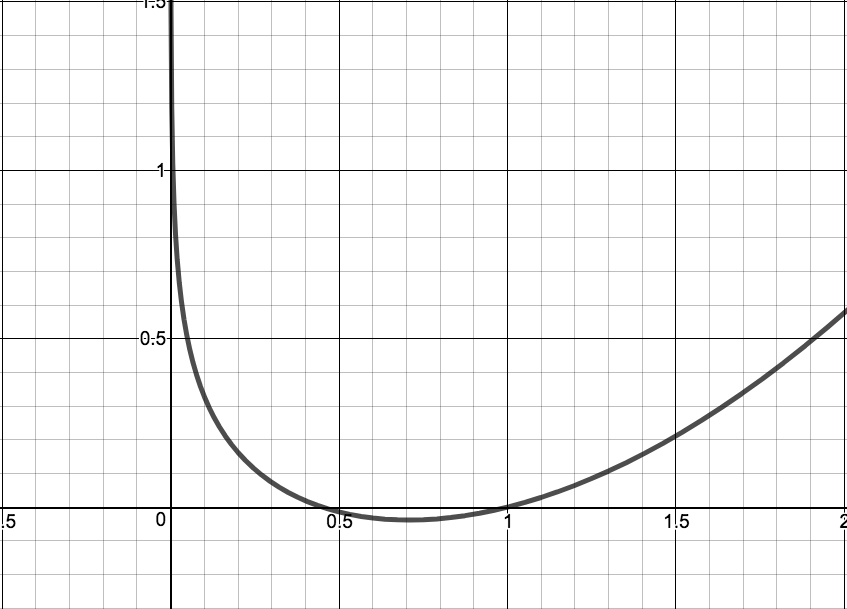
\includegraphics[height=1.5in]{./ApplicationsofExponentialandLogarithmicFunctionsGraphics/PURSUIT03.jpg}

\smallskip

$y(x) = \frac{1}{4} x^2-\frac{1}{4} \ln(x)-\frac{1}{4}$

\end{center}

\item The steady state current is 2 amps.

\addtocounter{enumi}{1}

\item  630 feet.

\item The linear regression on the data below is $y = 1.74899x + 0.70739$ with $r^{2} \approx 0.999995$.  

This is an excellent fit.

\scriptsize

\noindent \begin{tabular}{|l|r|r|r|r|r|r|r|r|r|r|} \hline
$x$ & 1 & 2 & 3 & 4 & 5 & 6 & 7 & 8 & 9 & 10 \\ 
\hline 
$\ln(N(x))$ & 2.4849 & 4.1897 & 5.9454 & 7.6967 & 9.4478 & 11.1988 & 12.9497 & 14.7006 & 16.4523 & 18.2025 \\ \hline
\end{tabular}

\normalsize

$N(x) = 2.02869(5.74879)^{x} = 2.02869e^{1.74899x}$ with $r^{2} \approx 0.999995$.  This is also an excellent fit and corresponds to our linearized model because $\ln(2.02869) \approx 0.70739$.

\item  \begin{enumerate}
\addtocounter{enumii}{1}

\item  The linearized model is: $\ln(L(x)) \approx 2.106 \ln(x) - 5.268$ with an $r^2 \approx  0.9914$.

\item  $L(x) = 0.005154 x^{2.106}$.  $L(90) \approx 67.3$ meaning the bottom $90 \%$ of wage earners take home $67.3 \%$ of the total national income.  Said differently, according to this model, the top $10 \%$ of wage earners take home $32.7 \%$ of the total national income. 



\item  We graph our answer to Example \ref{LorenzEx} in Section \ref{PowerFunctions}, $L(x) = 0.00027901x^{2.7738}$, below on the left.  Below on the right is the model we derived in this exercise. 

\begin{center}

\begin{tabular}{cc}

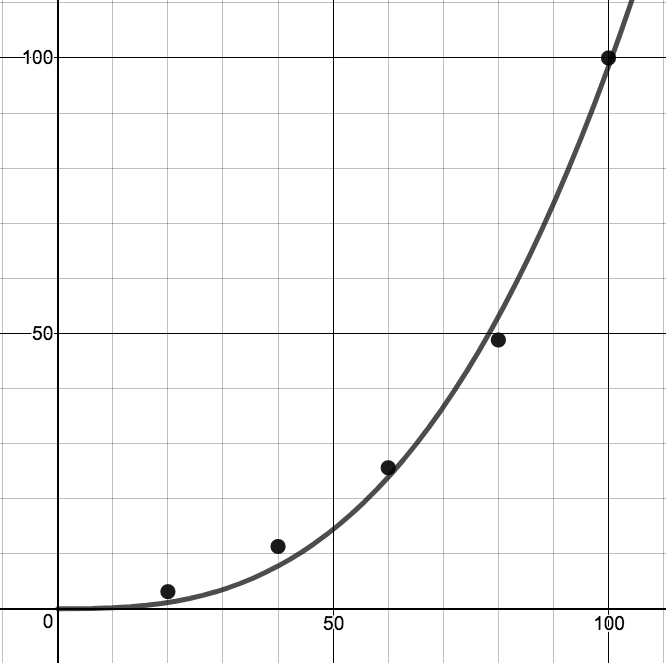
\includegraphics[height=1.5in]{./ApplicationsofExponentialandLogarithmicFunctionsGraphics/OldLorenzModel.jpg}  &

\hspace{1in}

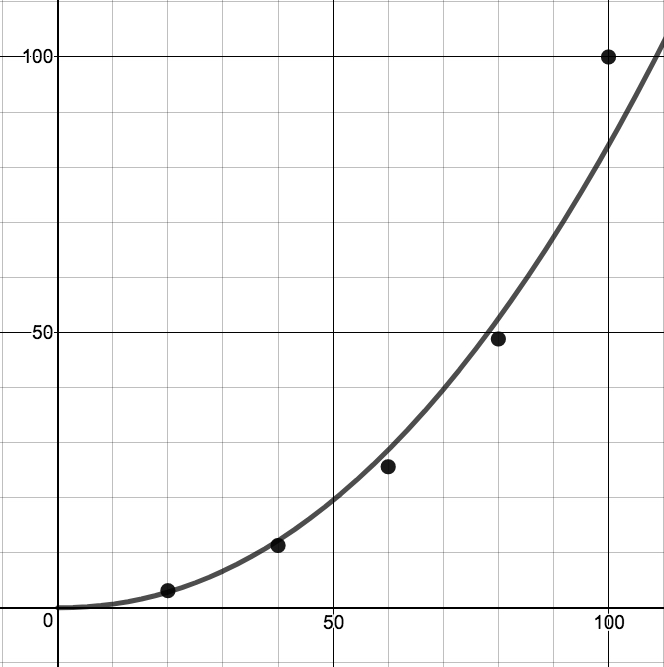
\includegraphics[height=1.5in]{./ApplicationsofExponentialandLogarithmicFunctionsGraphics/NewLorenzModel.jpg}  \\

 $L(x) = 0.00027901x^{2.7738}$

&

\hspace{1in}
$L(x) = 0.005154 x^{2.106}$ \\

\end{tabular}

\end{center}

\end{enumerate}


\item  \begin{enumerate}  \item   We get:  $y = 2895.06 (1.0147)^{x}$.  Graphing this along with our answer from Exercise \ref{PainesvillePopulationTwoPoint} over the interval $[0,60]$ shows that they are pretty close. From this model, $y(150) \approx 25840$ which once again overshoots the actual data value.

\item $P(150) \approx 18717$, so this model predicts 17,914 people in Painesville in 2010, a more conservative number than was recorded in the 2010 census.  As $t \rightarrow \infty$, $P(t) \rightarrow 18691$.  So the limiting population of Painesville based on this model is 18,691 people.

\enlargethispage{\baselineskip}

\end{enumerate}

\item \begin{enumerate}  \item  $y = \dfrac{242526}{1+874.63e^{-0.07113x}}$, where $x$ is the number of years since 1860.

\item  The plot of the data and the curve is below.

\centerline{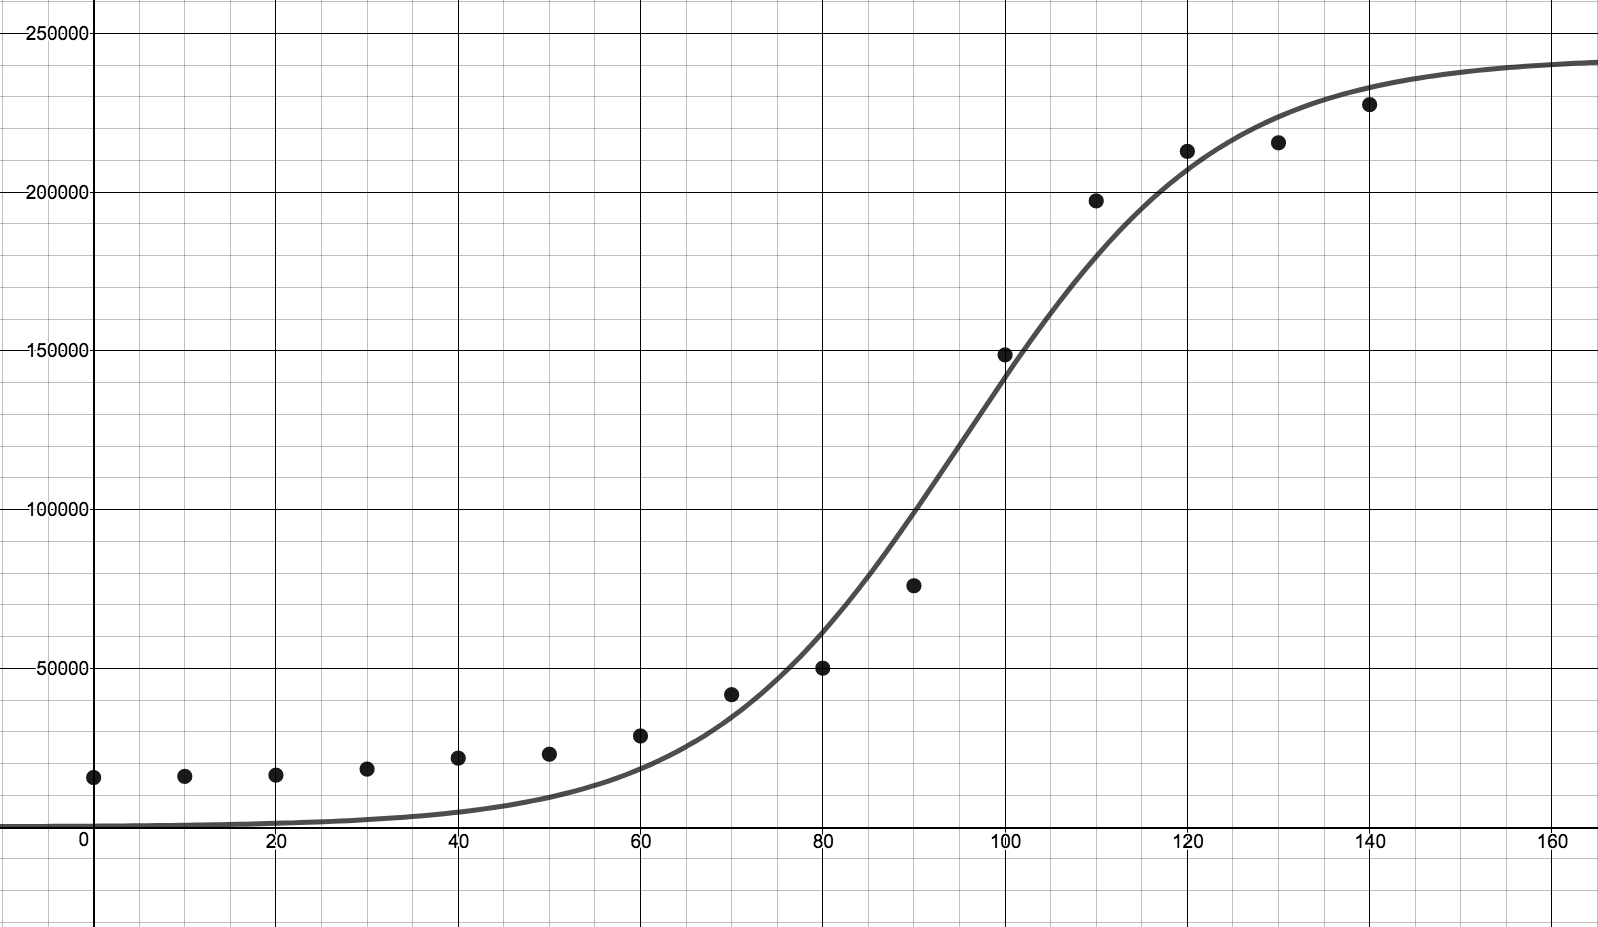
\includegraphics[height=2in]{./ApplicationsofExponentialandLogarithmicFunctionsGraphics/LAKECOUNTYLOGISTIC.jpg}} 

\item  $y(140) \approx 232884$, so this model predicts 232,884 people in Lake County in 2010.

\item  As $x \rightarrow \infty$, $y \rightarrow 242526$, so the limiting population of Lake County based on this model is 242,526 people.

\end{enumerate}

\end{enumerate}


\closegraphsfile